\documentclass{amsart}
\usepackage[foot]{amsaddr} % put addresses on first page

\usepackage{geometry}
\usepackage{graphicx,psfrag,epsf}
\usepackage{enumerate}
\usepackage{booktabs}
\usepackage{enumitem}
\usepackage{amsfonts}
\usepackage{mathtools}
\usepackage{amssymb}
\usepackage{amsmath}
\allowdisplaybreaks
\usepackage{longtable}
\usepackage{bigints}
\usepackage{siunitx}
\usepackage{amsthm}
\usepackage{soul}
\usepackage{color}

\usepackage{hyperref}
\usepackage[capitalise]{cleveref}
\newtheorem{theorem}{Theorem}[section]
\newtheorem{corollary}{Corollary}[theorem]
\newtheorem{lemma}[theorem]{Lemma}
%

\usepackage[numbers]{natbib}
\usepackage{url} % not crucial - just used below for the URL 
\usepackage{doi}

\title{Copula estimation using loss-based Bayesian Additive Regression Trees}
\author{**}
\date{\today}

\begin{document}

\maketitle

\section{Introduction}

\section{Model}
Let $Y_1$ and $Y_2$ be two continuous random variables and $X$ be a continuous random variable 
that might affect the relationship between $Y_1$ and $Y_2$. 
Then according to Sklar’s theorem there exists a unique copula such that:
\begin{equation}
    H_{X}(y_1,y_2\mid x; \theta, \alpha_1, \alpha_2) = C\{F_{Y_1\mid X}(y_1\mid x;\alpha_1),F_{Y_2\mid X}(y_2\mid x; \alpha_2)\mid x;\theta\}; \quad \forall (y_1,y_2) \in \mathbb{R}^2.
\end{equation}
This gives us the following
\begin{equation}
    h_{X}(y_1,y_2\mid x; \theta, \alpha_1, \alpha_2) = f_{Y_1\mid X}(y_1\mid x;\alpha_1)f_{Y_2\mid X}(y_2\mid x; \alpha_2)c(u_1,u_2\mid x;\theta),
\end{equation}
where
\begin{equation}\label{eq:emp_dist:Y}
    u_k = F_{Y_k\mid X}(y_k\mid x; \alpha_k)
\end{equation}
and $c(u_1,u_2\mid x;\theta)$ is conditional copula density function.

\subsection{Copula parameter estimation}

Let $\Phi_{\theta\mid x}(y_1, y_2)$ denote the standard bivariate normal distribution with correlation coefficient $\theta$ conditional on $X$. Then
the corresponding copula density function is given by:

\begin{equation}
    c(u_1,u_2\mid x;\theta) \coloneqq c_{\theta_x}(u_1, u_2) 
    = \frac{1}{\sqrt{|\Sigma|}} \exp\left( -\frac{1}{2}
    \begin{bmatrix}
    \Phi^{-1}(u_1) \\
    \Phi^{-1}(u_2)
    \end{bmatrix}^\top
    (\Sigma^{-1} - I)
    \begin{bmatrix}
    \Phi^{-1}(u_1) \\
    \Phi^{-1}(u_2)
    \end{bmatrix}
    \right)
\end{equation}

where

\[
\Sigma = \begin{bmatrix}
1 & \theta_x \\
\theta_x & 1
\end{bmatrix}
\]

and \( \Phi^{-1} \) is the inverse of the standard normal cumulative distribution function. Simplifying we get:

\begin{equation}
    c_{\theta_X}(u_1, u_2) = \frac{1}{\sqrt{1 - \theta_x^2}} \exp \left( -\frac{2\theta_x \Phi^{-1}(u_1) \Phi^{-1}(u_2) - \theta_x^2\left[\Phi^{-1}(u_1)^2 + \Phi^{-1}(u_2)^2\right]}{2(1 - \theta_x^2)} \right)
\end{equation}

Now, let $u_1 \coloneqq (u_{11}, u_{12}, \cdots, u_{1n})$ and $u_2 \coloneqq (u_{21}, u_{22}, \cdots, u_{2n})$ be a set of $n$ observations from a bivariate
Gaussian copula.


Then, the likelihood is given by:

\begin{align}
    \pi(U_1, U_2\mid X;\theta_x) &=\prod_{i=1}^n  
    \frac{1}{\sqrt{1 - \theta_{x_i}^2}} \exp \left( -\frac{2\theta_{x_i} \Phi^{-1}(u_{1i}) \Phi^{-1}(u_{2i}) - \theta_{x_i}^2\left[\Phi^{-1}(u_{1i})^2 + \Phi^{-1}(u_{2i})^2\right]}{2(1 - \theta_{x_i}^2)} \right)
\end{align}
where for a tree $T$ with terminal node values $M$
\begin{equation}
    \theta_{x_i} = g(x_i, T, M)
\end{equation}
Now, terminal node values $M \coloneqq (\mu_1, \mu_2, \cdots \mu_{n_L})$ has to
satisfy $\mu_j \in (-1,1)$. This leads to the issue of finding a suitable prior 
for $\mu_j$.

Note that the likelihood structure for a partition $\Omega_j$ of $x\coloneqq (x_1, x_2, \cdots, x_n)$

\begin{align}
    \pi(U_1, U_2\mid X;\theta_x) 
    &=(1 - \theta_{x}^2)^{-\frac{\#\Omega_j}{2}} \exp \left( -\frac{2A \theta_{x} - B\theta_{x}^2}{2(1 - \theta_{x}^2)} \right)
\end{align}
where $A \coloneqq \sum_{i\in \Omega_j}\Phi^{-1}(u_{1i}) \Phi^{-1}(u_{2i})$
and $B \coloneqq \left[\Phi^{-1}(u_{1i})^2 + \Phi^{-1}(u_{2i})^2\right]$. 

\subsubsection{Choice for $\mu_j$}
\begin{itemize}
    \item Jeffrey's prior \url{https://www2.stat.duke.edu/~berger/papers/bivariate.pdf}
    \item Simple uniform distribution in $(-1,1)$ 
    \item Transformed beta \url{https://academic.oup.com/jrsssa/article/145/2/237/7105492}
    \item Log-normal on $-\log(1-p^2)$
    \item Inverse-Gamma on $-\log(1-p^2)$
\end{itemize}
Note that for the first three choices, we only work with transformed beta distribution by 
selecting suitable hyper-parameters.

\subsection{Density of $\rho$}

Let $\kappa = -\log(1-p^2)$, then for $\rho \ge 0$
\begin{align}
	\rho & = \sqrt{1-\exp(-\kappa)}\coloneqq g(\kappa)
\end{align}

Now, let $0\le\kappa_1 < \kappa_2<\infty$, then

\begin{align}
	&g(\kappa_2) - g(\kappa_1)\\
	&=\sqrt{1-\exp(-\kappa_2)} - \sqrt{1-\exp(-\kappa_1)}\\
	&= \frac{(\sqrt{1-\exp(-\kappa_2)} - \sqrt{1-\exp(-\kappa_1)})(\sqrt{1-\exp(-\kappa_2)} + \sqrt{1-\exp(-\kappa_1)})}{(\sqrt{1-\exp(-\kappa_2)} + \sqrt{1-\exp(-\kappa_1)})}\\
	&= \frac{(1-\exp(-\kappa_2) - 1+\exp(-\kappa_1))}{(\sqrt{1-\exp(-\kappa_2)} + \sqrt{1-\exp(-\kappa_1)})}\\
	&= \frac{(\exp(-\kappa_1)-\exp(-\kappa_2))}{(\sqrt{1-\exp(-\kappa_2)} + \sqrt{1-\exp(-\kappa_1)})}\\
	&= \frac{(\exp(\kappa_2)-\exp(-\kappa_1))}
	{(\exp(\kappa_2)\exp(-\kappa_1))(\sqrt{1-\exp(-\kappa_2)} + \sqrt{1-\exp(-\kappa_1)})} >0.
\end{align}
Therefore it is monotone and increasing.

Now, for $\rho \ge 0$ the density is given by
\begin{align}
	f_{\rho}(\rho)&=f_{\kappa}(\kappa)\left|\frac{d \kappa}{d \rho}\right|\\
	&=f_{\kappa}\left(-\log(1-p^2)\right)\frac{2\rho}{1-\rho^2}
\end{align}
Therefore for log-normal distribution
\begin{equation}
	f_{\rho}(\rho)
	= \frac{1}{\sqrt{2\pi\sigma^2}(-\log(1-\rho^2))} 
	\exp\left(-\frac{(\log(-\log(1-\rho^2))-\mu)^2}{2\sigma^2}\right)
	\cdot \frac{2\rho}{1-\rho^2}
\end{equation}
Similarly, we can derive the expression $\rho<0$ using the relation
$\rho = -\sqrt{1-\exp(-\kappa)}$. This gives us the following
symmetric density function
\begin{equation}
	f_{\rho}(\rho)
	= \frac{\sqrt{2}|\rho|}{\sqrt{\pi}\sigma(1-\rho^2)(-\log(1-\rho^2))} 
	\exp\left(-\frac{(\log(-\log(1-\rho^2))-\mu)^2}{2\sigma^2}\right)
\end{equation}

\paragraph{Continuity at 0} To show the continuity of the density function at 0 we first need to show that the limit $f_{\rho}(0)$
exists.

Since,

\begin{align}
	\lim_{\rho\to 0}f_{\rho}(\rho)
	&= \lim_{\rho\to 0}\left[\frac{\sqrt{2}|\rho|}{\sqrt{\pi}\sigma(1-\rho^2)(-\log(1-\rho^2))} 
	\exp\left(-\frac{(\log(-\log(1-\rho^2))-\mu)^2}{2\sigma^2}\right)\right]\\
	&= \frac{\sqrt{2}}{\sqrt{\pi}\sigma}\lim_{\rho\to 0}\left[\frac{|\rho|}{(1-\rho^2)} \right]
	\lim_{\rho\to 0}\left[\frac{1}{(-\log(1-\rho^2))} 
	\exp\left(-\frac{(\log(-\log(1-\rho^2))-\mu)^2}{2\sigma^2}\right)\right]
\end{align}
The limit $\lim_{\rho\to 0}\left[\frac{|\rho|}{(1-\rho^2)} \right]$ exists and equal to zero. For the remaining part we use change of variables.

\begin{align}
	&\lim_{\rho\to 0}\left[\frac{1}{(-\log(1-\rho^2))} 
	\exp\left(-\frac{(\log(-\log(1-\rho^2))-\mu)^2}{2\sigma^2}\right)\right]\\
	& = \lim_{\kappa\to 0}\left[\frac{1}{\kappa} 
	\exp\left(-\frac{(\log(\kappa)-\mu)^2}{2\sigma^2}\right)\right]\\
	& = \lim_{\eta\to -\infty}\left[\frac{1}{\exp(\eta)} 
	\exp\left(-\frac{(\eta-\mu)^2}{2\sigma^2}\right)\right]\\
	& = \lim_{\eta\to -\infty}\left[\frac{1}{\exp(\eta)} 
	\exp\left(-\frac{(\eta-\mu)^2}{2\sigma^2}\right)\right]\quad \text{TB: this holds for finite limits need to verify infinite}\\
	& = \lim_{\eta\to -\infty}\left[ 
	\exp\left(-\frac{(\eta-\mu)^2}{2\sigma^2}-\eta\right)\right] = 0
\end{align}
Since the density function is symmetric around 0, proceeding like before we can show that
\begin{equation}
	\lim_{\rho\to 0+}f_{\rho}(\rho) = \lim_{\rho\to 0-}f_{\rho}(\rho) = 0
\end{equation}

Now, for inverse-gamma distribution, the density of $\kappa$ is given by:
\begin{equation}
	f_{\kappa}(\kappa)= \frac{b^{a}}{\Gamma(a)}
	\kappa^{-a-1}\exp(-b/\kappa)
\end{equation}
Therefore, the density of $\rho$ is given by:
\begin{equation}
	f_{\rho}(\rho) = \frac{2b^{a}|\rho|}{\Gamma(a)(1-\rho^2)}
	(-\log(1-p^2))^{-a-1}\exp\left(-\frac{b}{-\log(1-p^2)}\right)
\end{equation}
Like before, we can show that the function is continuous at 0.

\begin{figure}[ht]
	\centering
	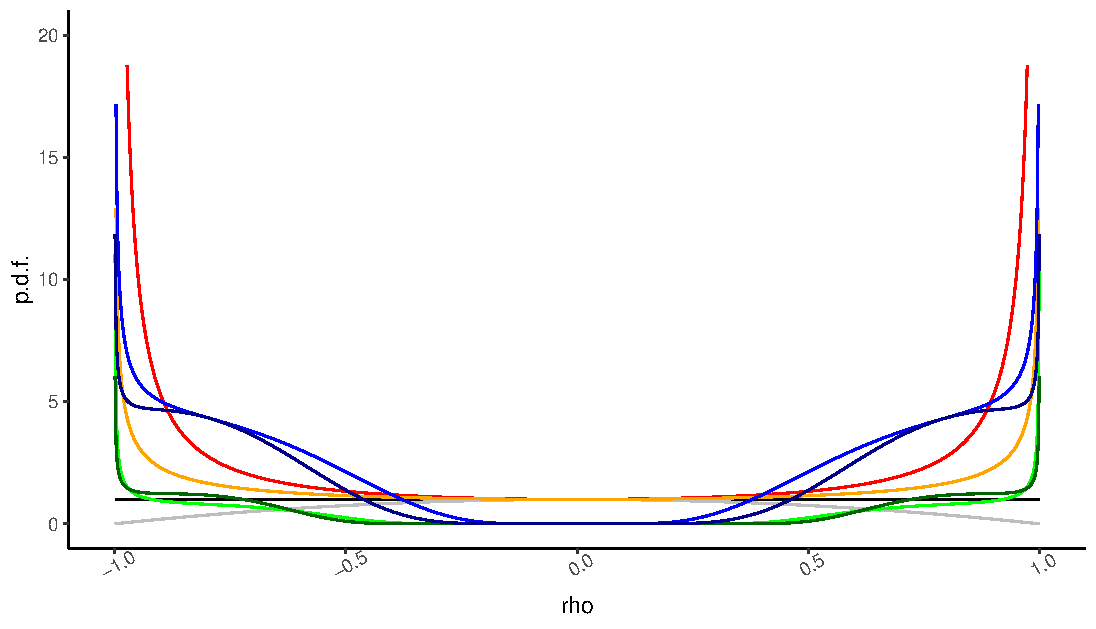
\includegraphics[width=0.85\linewidth]{prior_comparison.pdf}
	\caption{Different probability density functions for $\mu_{ij}$ a)black for uniform distribution,
	b)grey for Beta(2,2),
	c)red for Jeffrey's prior,
	d)orange for Beta(0.5,0.5),
	e)green for inverse-gamma (1,1),
	f)dark green for inverse-gamma (2,2),
	g)blue for log-normal (0,1) and
	h)dark blue for log-normal (0, 0.8)}
	\label{fig:sim-prior}
\end{figure}


\section{Simulation Studies}

We consider 5 different test cases so that
\begin{itemize}
    \item True $\theta_x$ has a tree structure with respect to $x$
    \item True $\theta_x$ is monotone with respect to $x$ such that 
    \begin{equation}
        \theta_x = 0.5 + 0.2 \sin(3x) + 0.3x^2
    \end{equation}
    \item True $\theta_x$ is convex with respect to $x$ such that 
    \begin{equation}
        \theta_x = 0.6 + 0.3 \sin(3x)
    \end{equation}
    \item True $\theta_x$ is concave with respect to $x$ such that 
    \begin{equation}
        \theta_x = 0.9 - 0.3 \sin(3x)
    \end{equation}
    \item True $\theta_x$ non-convex and non-monotone with respect to $x$ such that 
    \begin{equation}
        \theta_x = 0.7 - 0.3 \sin(2x) + 0.2 \sin(4x) + 0.3 x^2
    \end{equation}
\end{itemize}

% Frank and Clayton with right likelihood
% with Gaussian likelihood
% weak dependence


\begin{table}[ht]
\centering
\begin{tabular}{l|l|ccc}
  \toprule
 & Prior on $\mu_{ij}$ & RMSE & CI length & CI coverage \\ 
  \midrule
Case 1 & IG(1,1) & 0.0036 & 0.1163 & 0.622 \\ 
  & IG(2,2) & 0.0051 & \textbf{0.0921} & 0.488 \\ 
  & LN(0,0.8) & \textbf{0.0029} & 0.1037 & 0.626 \\ 
  & LN(0,1) & 0.0046 & 0.1673 & \textbf{0.950} \\ 
  & Jeffrey & 0.0034 & 0.1265 & 0.704 \\ 
  & Beta(0.5,0.5) & 0.0037 & 0.1359 & 0.652 \\ 
  & Beta(2,2) & 0.0041 & 0.1214 & 0.508 \\ 
  & Uniform & 0.0072 & 0.1394 & 0.658 \\ 
   \midrule
Case 2 & IG(1,1) & 0.0024 & \textbf{0.1396} & 0.586 \\ 
  & IG(2,2) & \textbf{0.0012} & 0.1696 & \textbf{0.996} \\ 
  & LN(0,0.8) & 0.0017 & 0.1670 & 0.882 \\ 
  & LN(0,1) & 0.0019 & 0.1524 & 0.906 \\ 
  & Jeffrey & 0.0034 & 0.1561 & 0.900 \\ 
  & Beta(0.5,0.5) & 0.0031 & 0.1496 & 0.740 \\ 
  & Beta(2,2) & 0.0031 & 0.1696 & 0.810 \\ 
  & Uniform & 0.0020 & 0.1510 & 0.986 \\ 
   \midrule
Case 3 & IG(1,1) & 0.0014 & 0.1134 & \textbf{0.884} \\ 
  & IG(2,2) & 0.0017 & 0.1062 & 0.772 \\ 
  & LN(0,0.8) & \textbf{0.0013} & 0.1137 & 0.792 \\ 
  & LN(0,1) & 0.0021 & \textbf{0.0992} & 0.736 \\ 
  & Jeffrey & 0.0019 & 0.1153 & 0.754 \\ 
  & Beta(0.5,0.5) & \textbf{0.0013} & 0.1167 & 0.826 \\ 
  & Beta(2,2) & 0.0022 & 0.1048 & 0.640 \\ 
  & Uniform & 0.0017 & 0.1221 & 0.738 \\ 
   \midrule
Case 4 & IG(1,1) & \textbf{0.0013} & \textbf{0.1393} & 0.856 \\ 
  & IG(2,2) & 0.0015 & 0.1583 & 0.920 \\ 
  & LN(0,0.8) & 0.0017 & 0.1690 & 0.934 \\ 
  & LN(0,1) & 0.0028 & 0.1519 & 0.930 \\ 
  & Jeffrey & 0.0027 & 0.1520 & 0.892 \\ 
  & Beta(0.5,0.5) & 0.0024 & 0.1568 & \textbf{0.938} \\ 
  & Beta(2,2) & 0.0019 & 0.1642 & 0.900 \\ 
  & Uniform & 0.0021 & 0.1832 & 0.930 \\ 
   \midrule
Case 5 & IG(1,1) & 0.0007 & 0.1167 & \textbf{1.000} \\ 
  & IG(2,2) & 0.0007 & 0.1111 & 0.834 \\ 
  & LN(0,0.8) & \textbf{0.0006} & 0.1371 & \textbf{1.000} \\ 
  & LN(0,1) & 0.0007 & \textbf{0.1045} & \textbf{1.000} \\ 
  & Jeffrey & 0.0007 & 0.1265 & \textbf{1.000} \\ 
  & Beta(0.5,0.5) & 0.0011 & 0.1284 & 0.808 \\ 
  & Beta(2,2) & 0.0009 & 0.1434 & 0.894 \\ 
  & Uniform & 0.0059 & 0.1573 & 0.932 \\ 
   \bottomrule
\end{tabular}
\end{table}

\begin{figure}[ht]
    \centering
    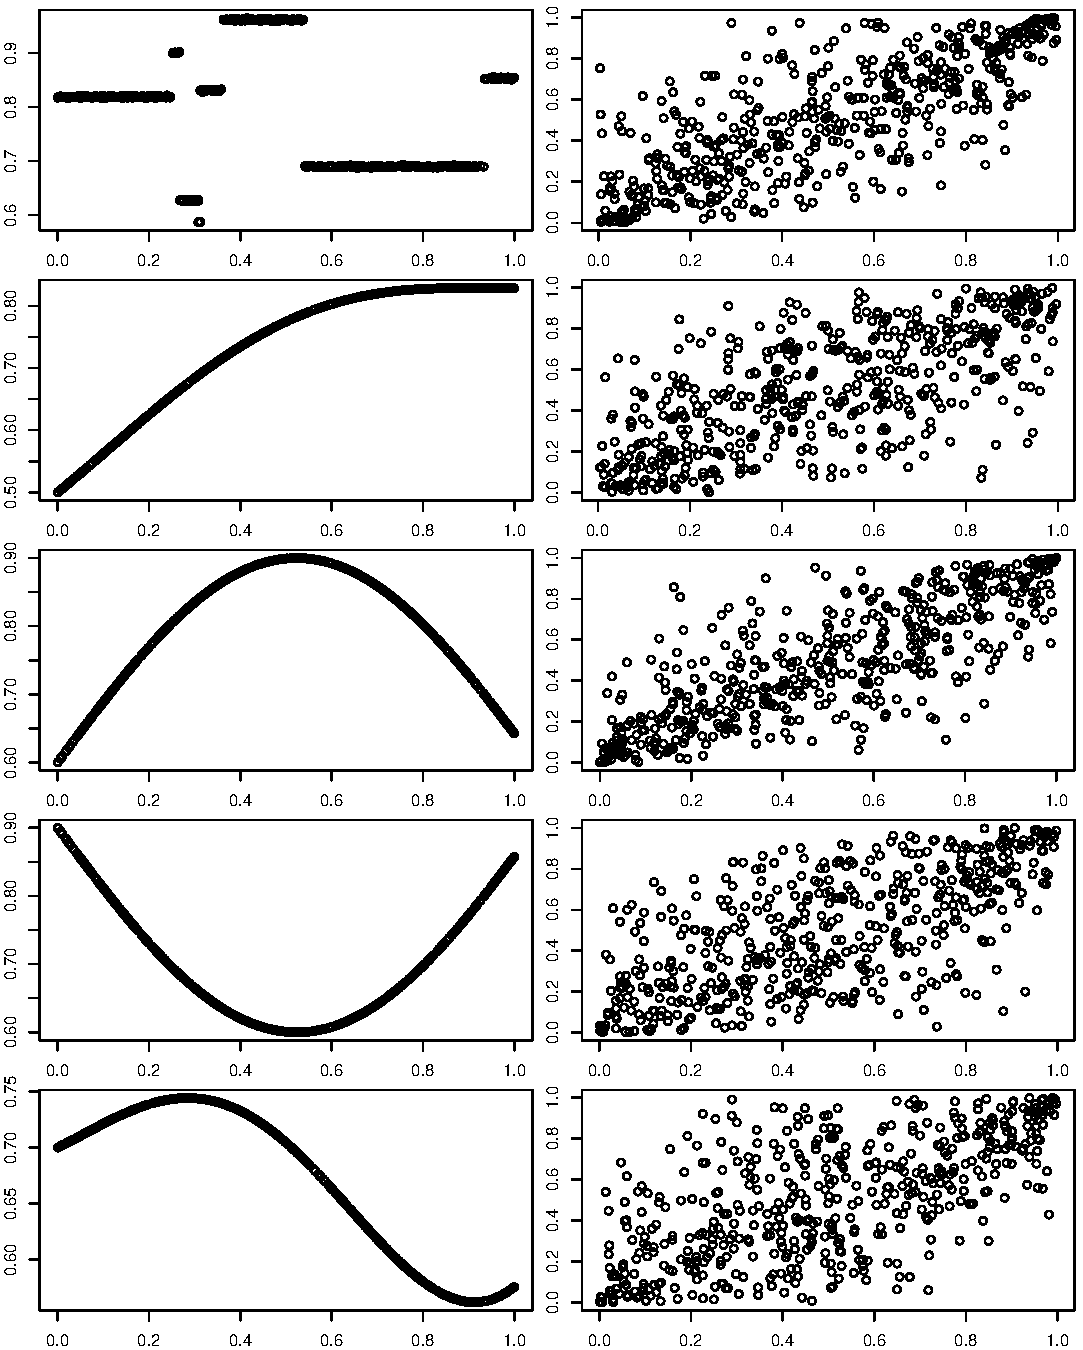
\includegraphics[width=0.95\linewidth]{true_rho_copula.pdf}
    \caption{Simulated $\rho$ and corresponding copula}
    \label{fig:sim-dat}
\end{figure}

\begin{figure}[ht]
	\centering
	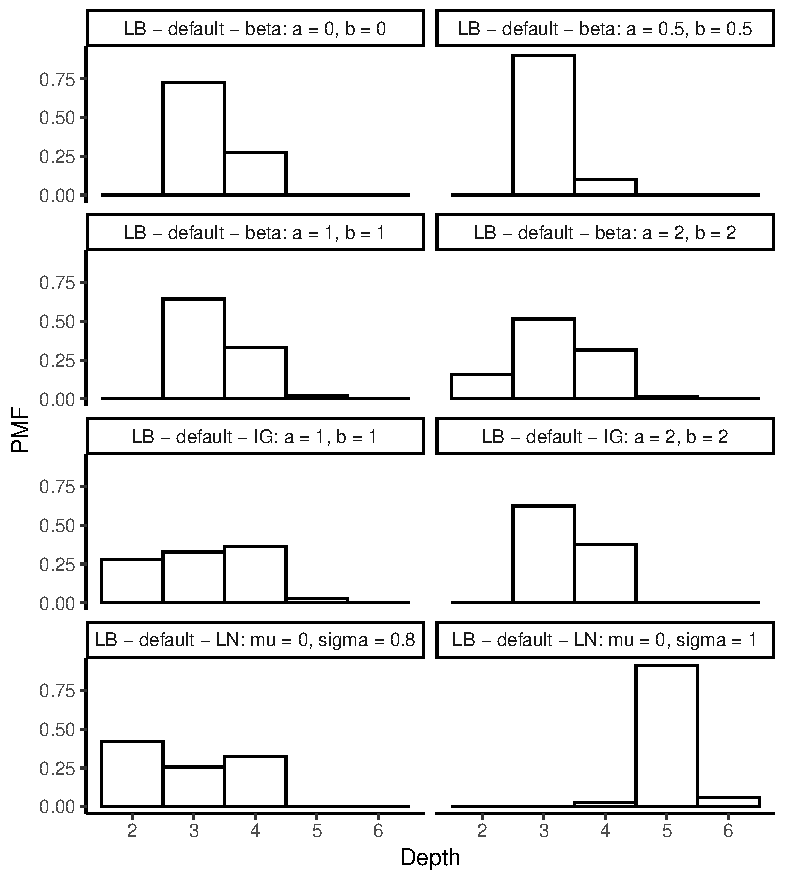
\includegraphics[width=0.95\linewidth]{hist_depth_1.pdf}
	\caption{Histogram of depth}
	\label{fig:hist:depth:1}
\end{figure}

\begin{figure}[ht]
	\centering
	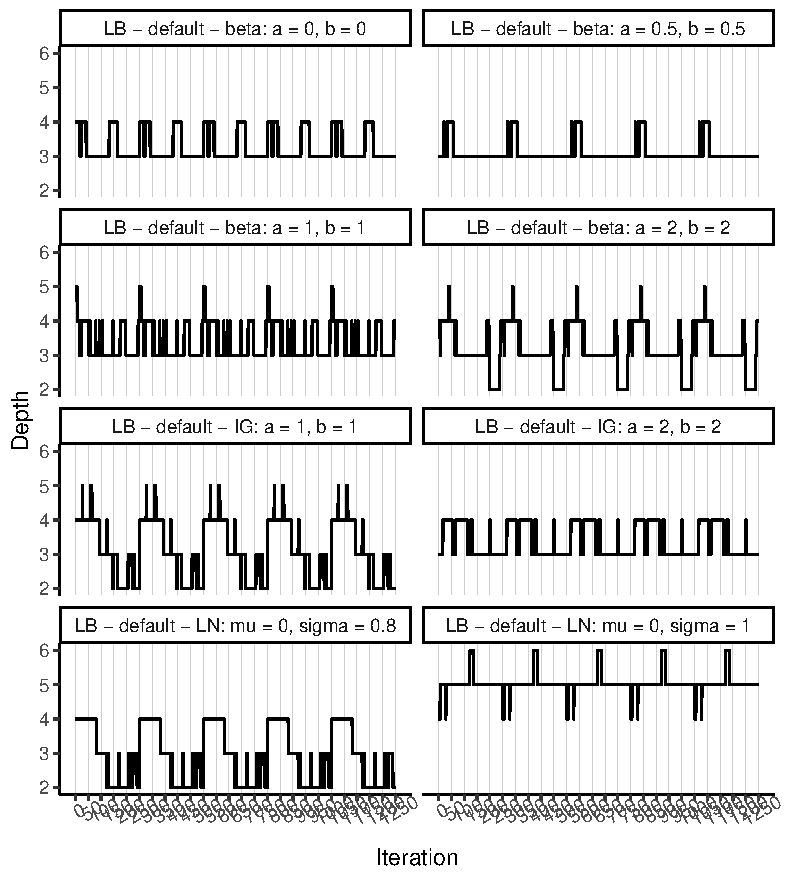
\includegraphics[width=0.95\linewidth]{trace_depth_1.pdf}
	\caption{Trace of depth}
	\label{fig:trace:depth:1}
\end{figure}

\begin{figure}[ht]
	\centering
	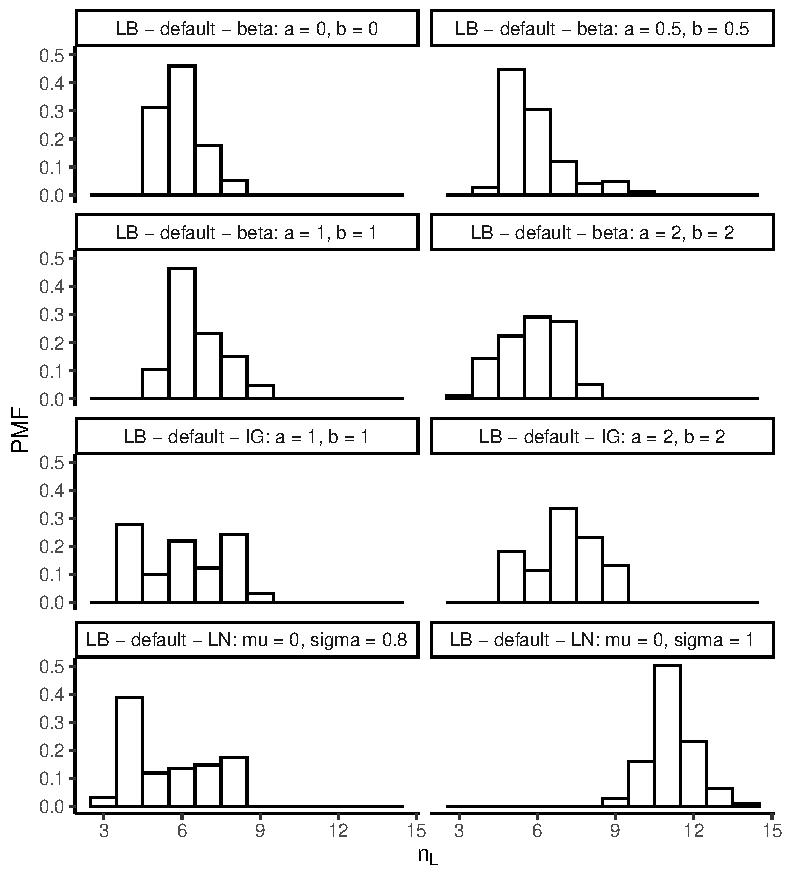
\includegraphics[width=0.95\linewidth]{hist_nl_1.pdf}
	\caption{Histogram of $n_L$}
	\label{fig:hist:nl:1}
\end{figure}

\begin{figure}[ht]
	\centering
	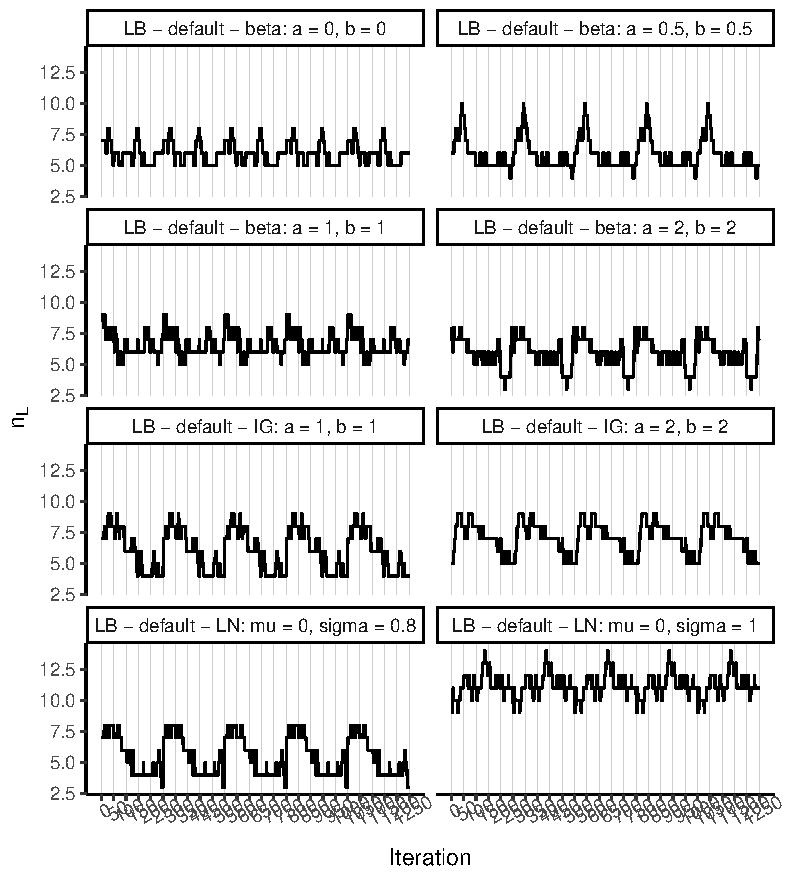
\includegraphics[width=0.95\linewidth]{trace_nl_1.pdf}
	\caption{Trace of $n_L$}
	\label{fig:trace:nl:1}
\end{figure}
\iffalse
\begin{figure}[ht]
	\centering
	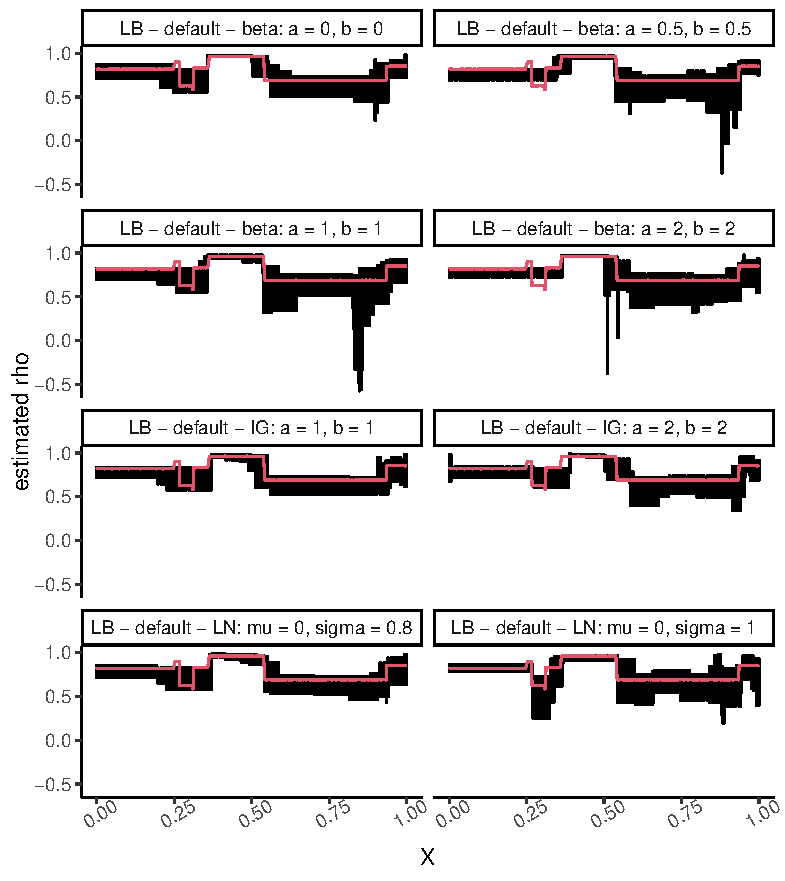
\includegraphics[width=0.95\linewidth]{mcmc_rho_1.pdf}
	\caption{MCMC of $\rho$}
	\label{fig:mcmc:rho:1}
\end{figure}
\fi
\begin{figure}[ht]
	\centering
	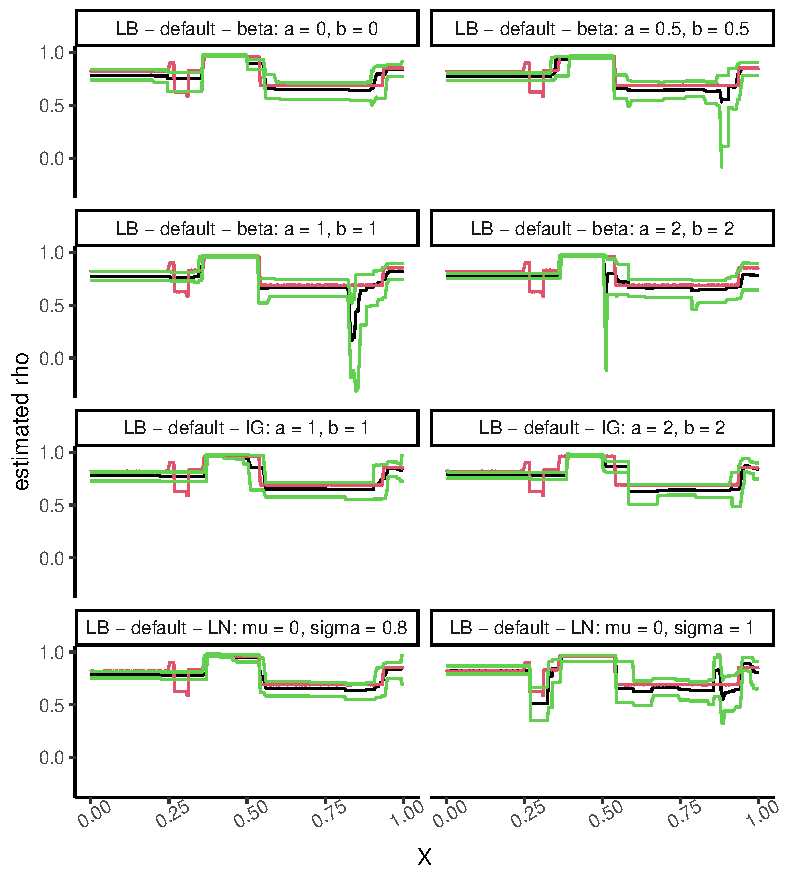
\includegraphics[width=0.95\linewidth]{predicted_rho_1.pdf}
	\caption{Estimated $\rho$ and credible intervals}
	\label{fig:pred:rho:1}
\end{figure}

\begin{figure}[ht]
	\centering
	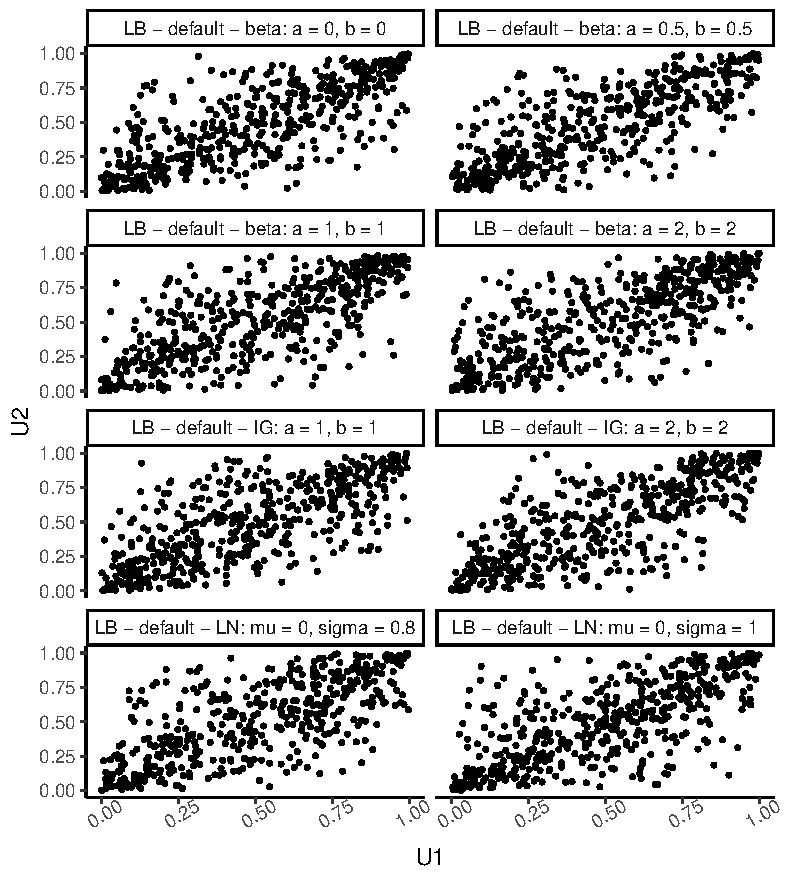
\includegraphics[width=0.95\linewidth]{simulated_copula_1.pdf}
	\caption{Predicted copula with estimated $\rho$}
	\label{fig:sim:copula:1}
\end{figure}

%
\begin{figure}[ht]
	\centering
	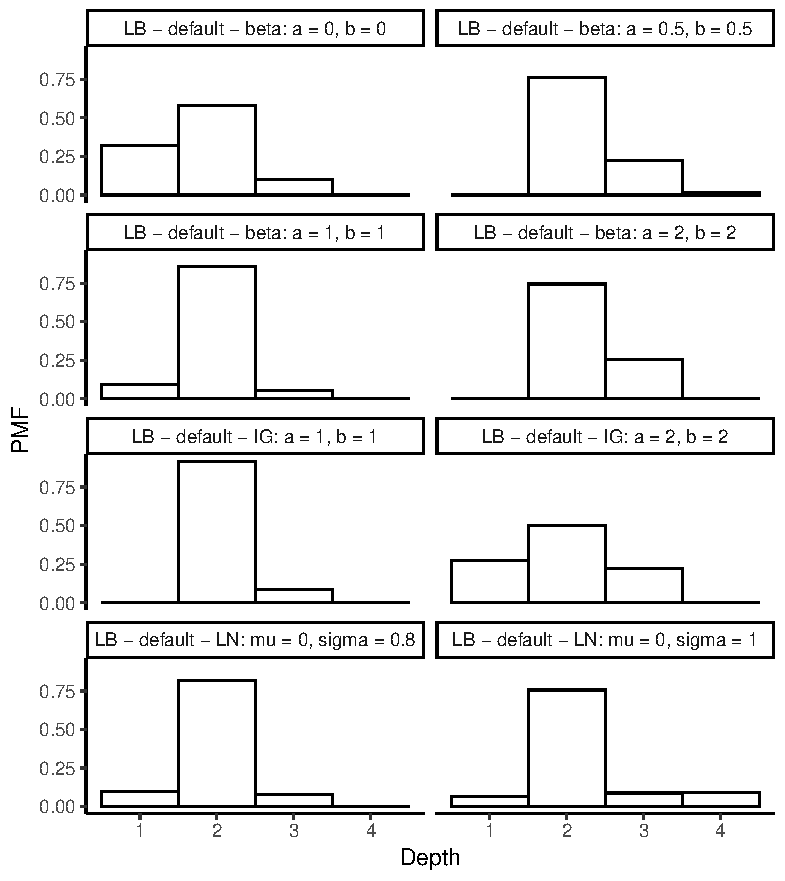
\includegraphics[width=0.95\linewidth]{hist_depth_2.pdf}
	\caption{Histogram of depth}
	\label{fig:hist:depth:2}
\end{figure}

\begin{figure}[ht]
	\centering
	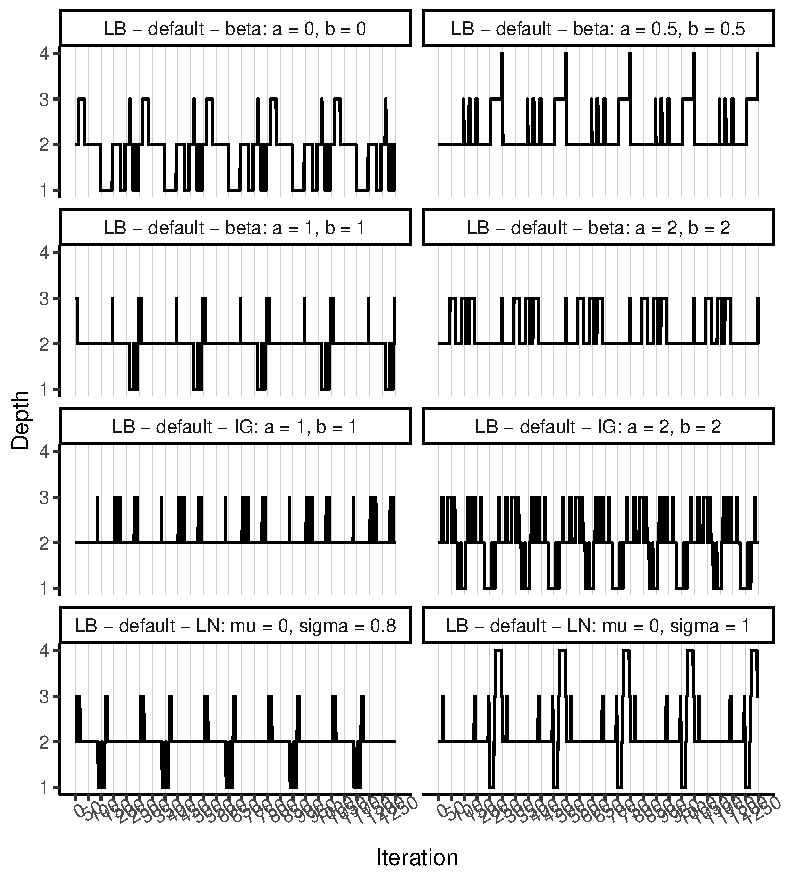
\includegraphics[width=0.95\linewidth]{trace_depth_2.pdf}
	\caption{Trace of depth}
	\label{fig:trace:depth:2}
\end{figure}

\begin{figure}[ht]
	\centering
	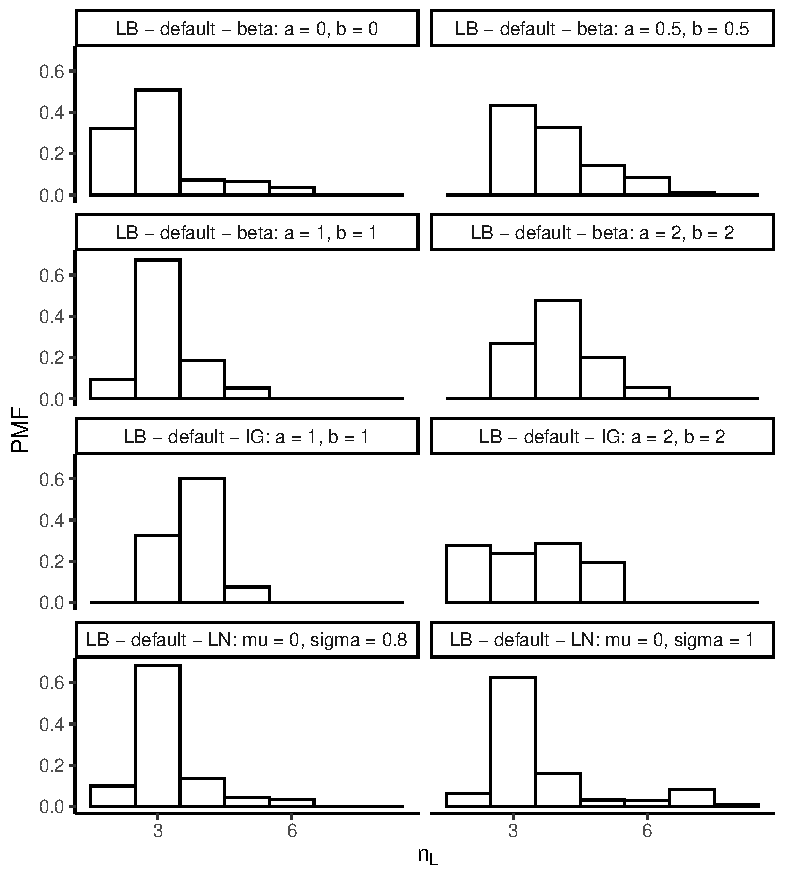
\includegraphics[width=0.95\linewidth]{hist_nl_2.pdf}
	\caption{Histogram of $n_L$}
	\label{fig:hist:nl:2}
\end{figure}

\begin{figure}[ht]
	\centering
	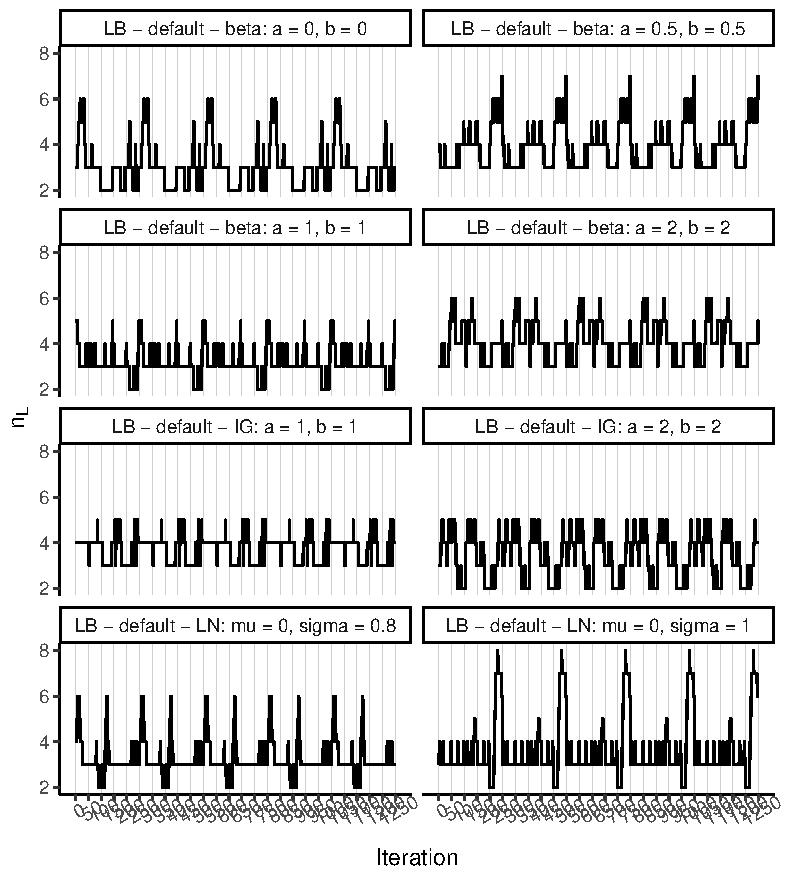
\includegraphics[width=0.95\linewidth]{trace_nl_2.pdf}
	\caption{Trace of $n_L$}
	\label{fig:trace:nl:2}
\end{figure}
\iffalse
\begin{figure}[ht]
	\centering
	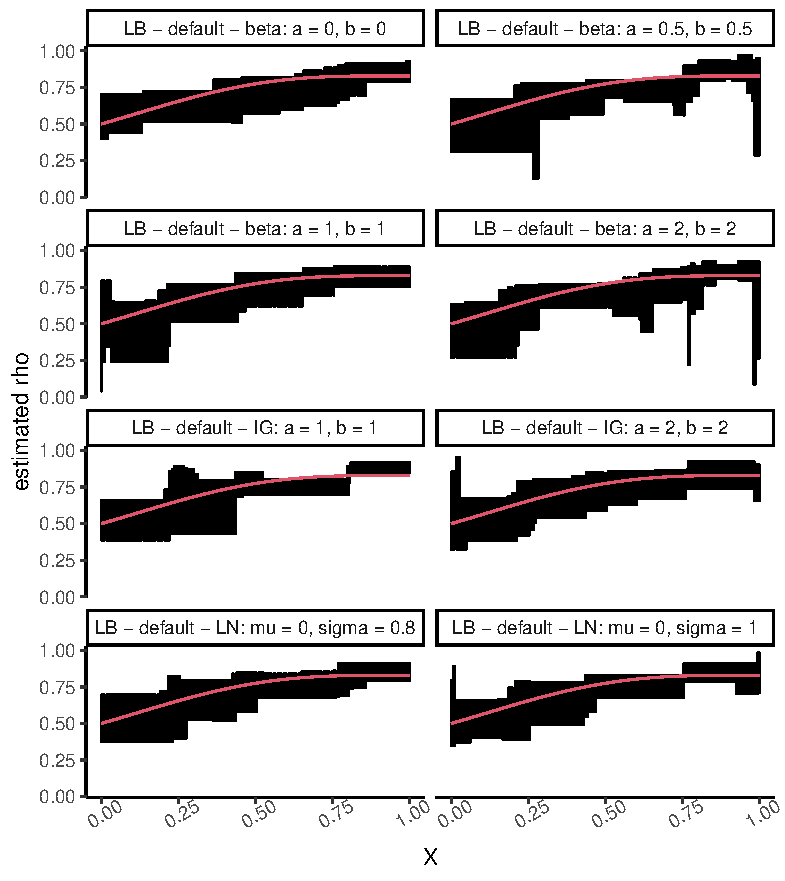
\includegraphics[width=0.95\linewidth]{mcmc_rho_2.pdf}
	\caption{MCMC of $\rho$}
	\label{fig:mcmc:rho:2}
\end{figure}
\fi
\begin{figure}[ht]
	\centering
	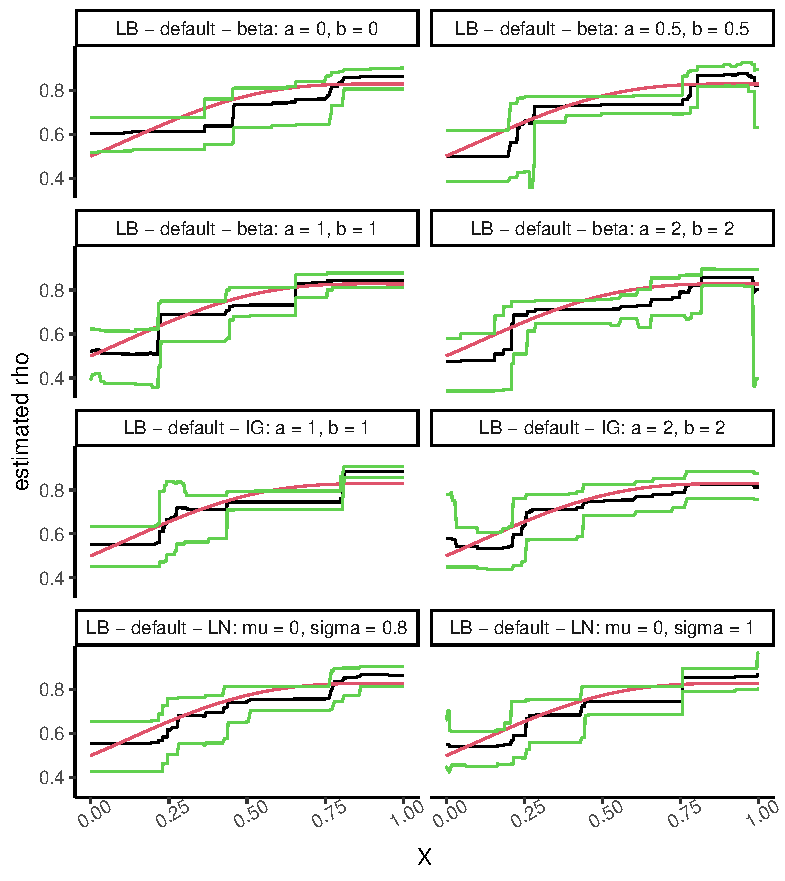
\includegraphics[width=0.95\linewidth]{predicted_rho_2.pdf}
	\caption{Estimated $\rho$ and credible intervals}
	\label{fig:pred:rho:2}
\end{figure}

\begin{figure}[ht]
	\centering
	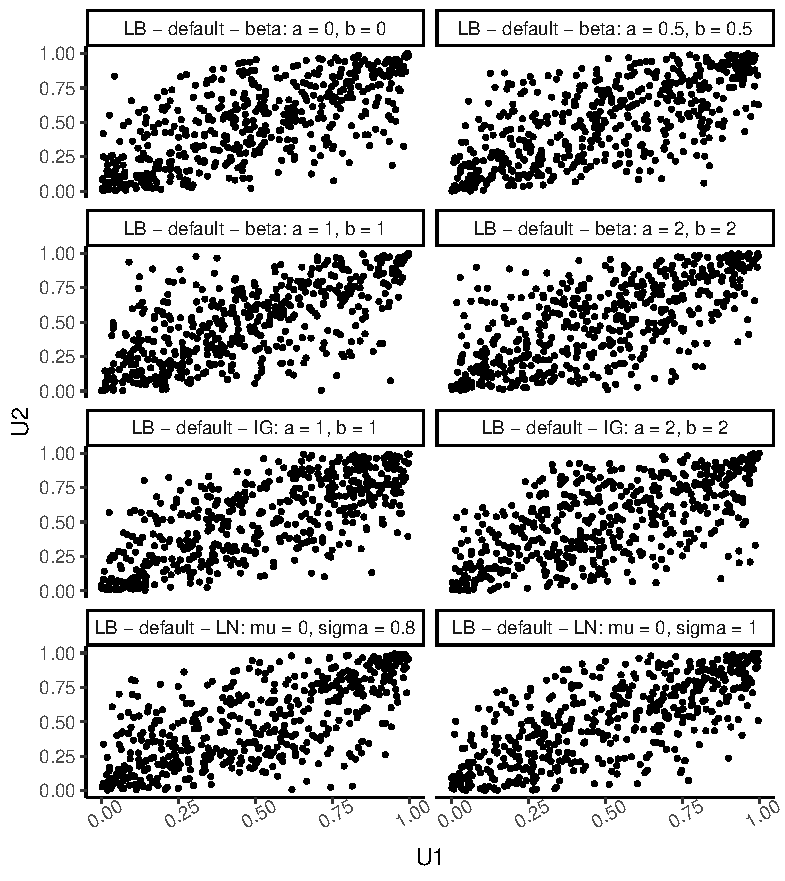
\includegraphics[width=0.95\linewidth]{simulated_copula_2.pdf}
	\caption{Predicted copula with estimated $\rho$}
	\label{fig:sim:copula:2}
\end{figure}

%
\begin{figure}[ht]
	\centering
	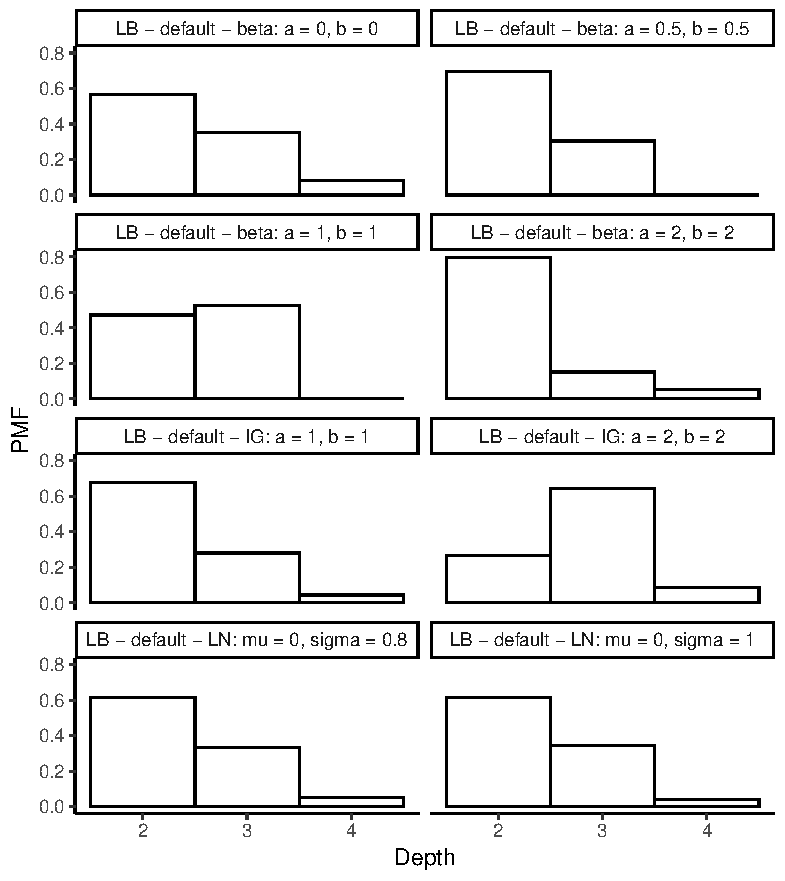
\includegraphics[width=0.95\linewidth]{hist_depth_3.pdf}
	\caption{Histogram of depth}
	\label{fig:hist:depth:3}
\end{figure}

\begin{figure}[ht]
	\centering
	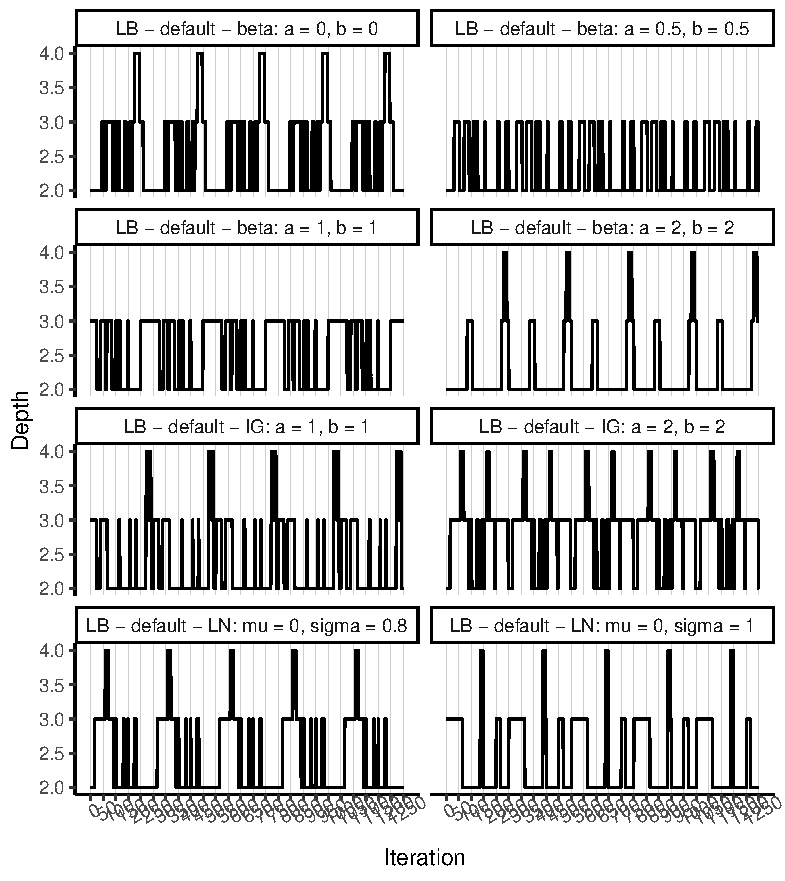
\includegraphics[width=0.95\linewidth]{trace_depth_3.pdf}
	\caption{Trace of depth}
	\label{fig:trace:depth:3}
\end{figure}

\begin{figure}[ht]
	\centering
	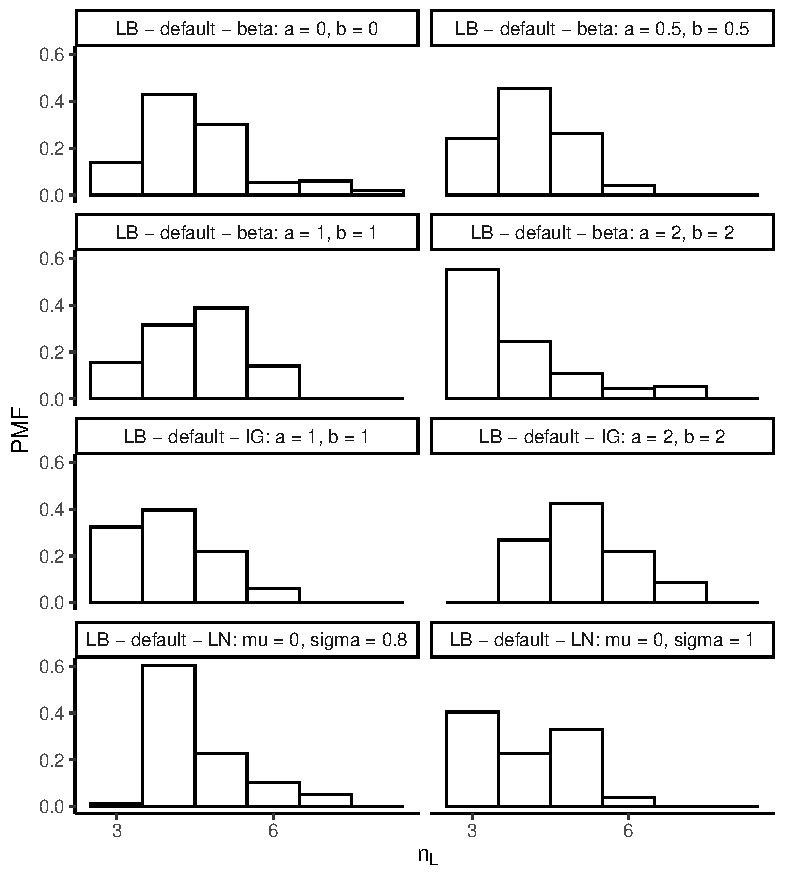
\includegraphics[width=0.95\linewidth]{hist_nl_3.pdf}
	\caption{Histogram of $n_L$}
	\label{fig:hist:nl:3}
\end{figure}

\begin{figure}[ht]
	\centering
	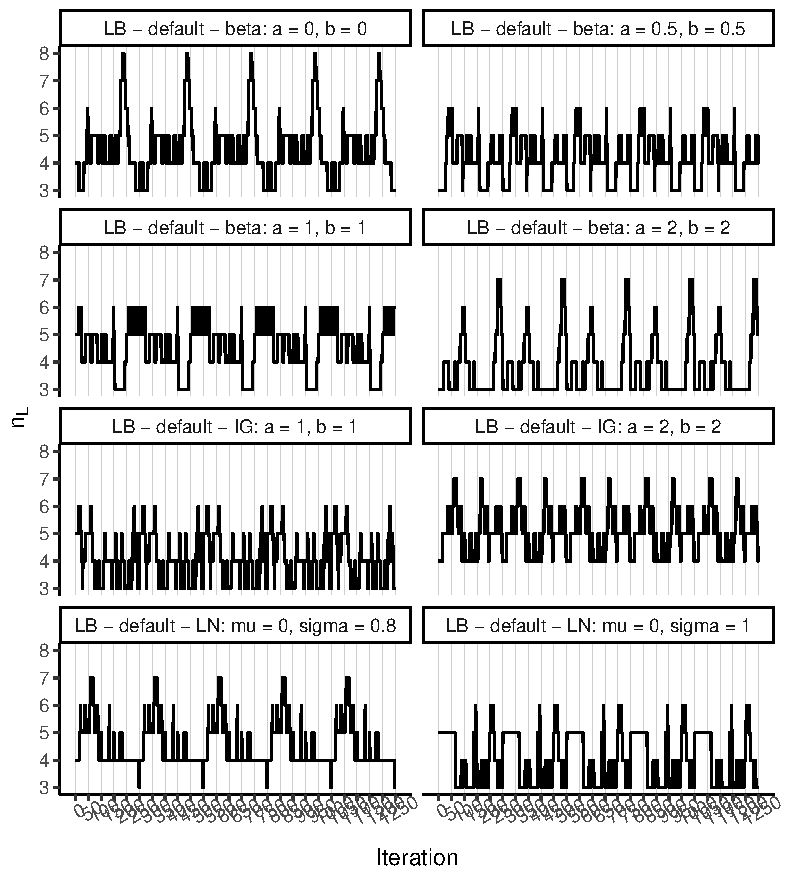
\includegraphics[width=0.95\linewidth]{trace_nl_3.pdf}
	\caption{Trace of $n_L$}
	\label{fig:trace:nl:3}
\end{figure}
\iffalse
\begin{figure}[ht]
	\centering
	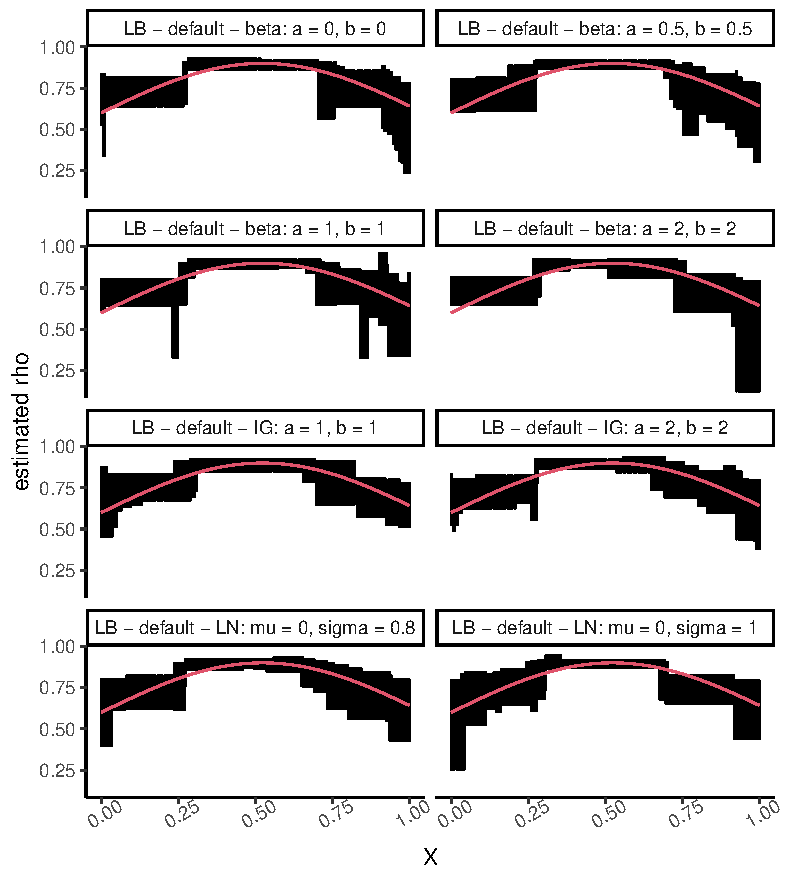
\includegraphics[width=0.95\linewidth]{mcmc_rho_3.pdf}
	\caption{MCMC of $\rho$}
	\label{fig:mcmc:rho:3}
\end{figure}
\fi
\begin{figure}[ht]
	\centering
	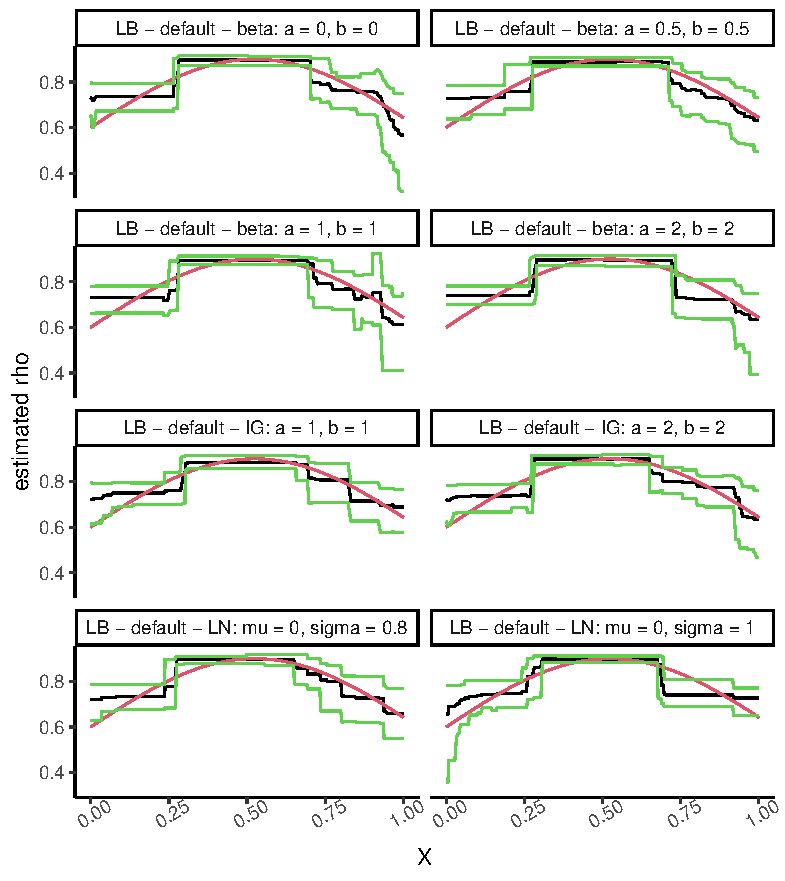
\includegraphics[width=0.95\linewidth]{predicted_rho_3.pdf}
	\caption{Estimated $\rho$ and credible intervals}
	\label{fig:pred:rho:3}
\end{figure}

\begin{figure}[ht]
	\centering
	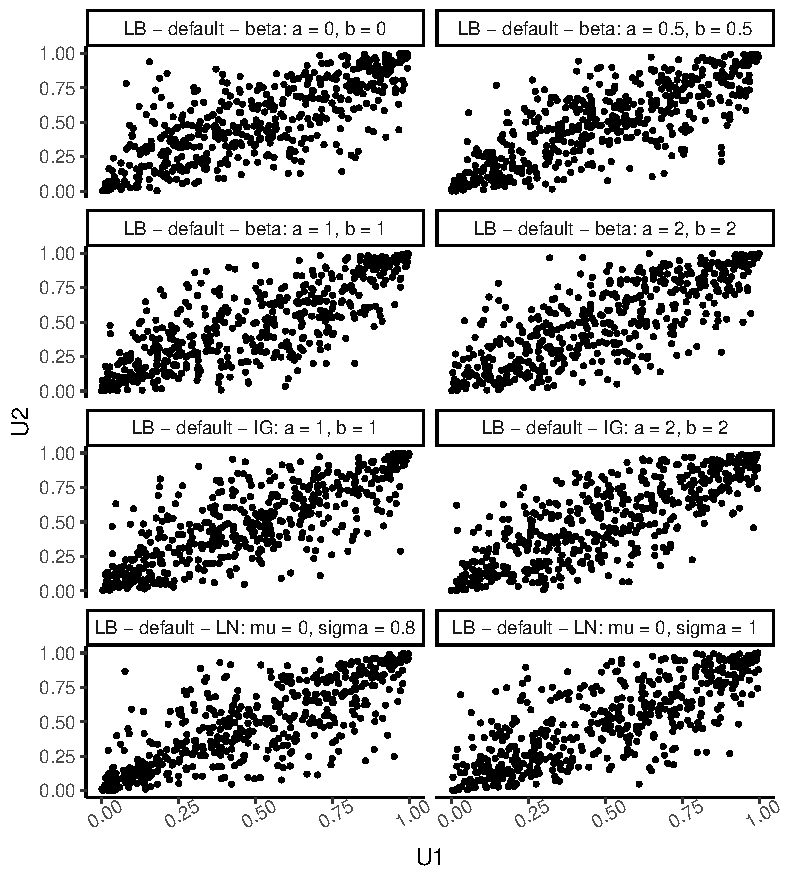
\includegraphics[width=0.95\linewidth]{simulated_copula_3.pdf}
	\caption{Predicted copula with estimated $\rho$}
	\label{fig:sim:copula:3}
\end{figure}

%
\begin{figure}[ht]
	\centering
	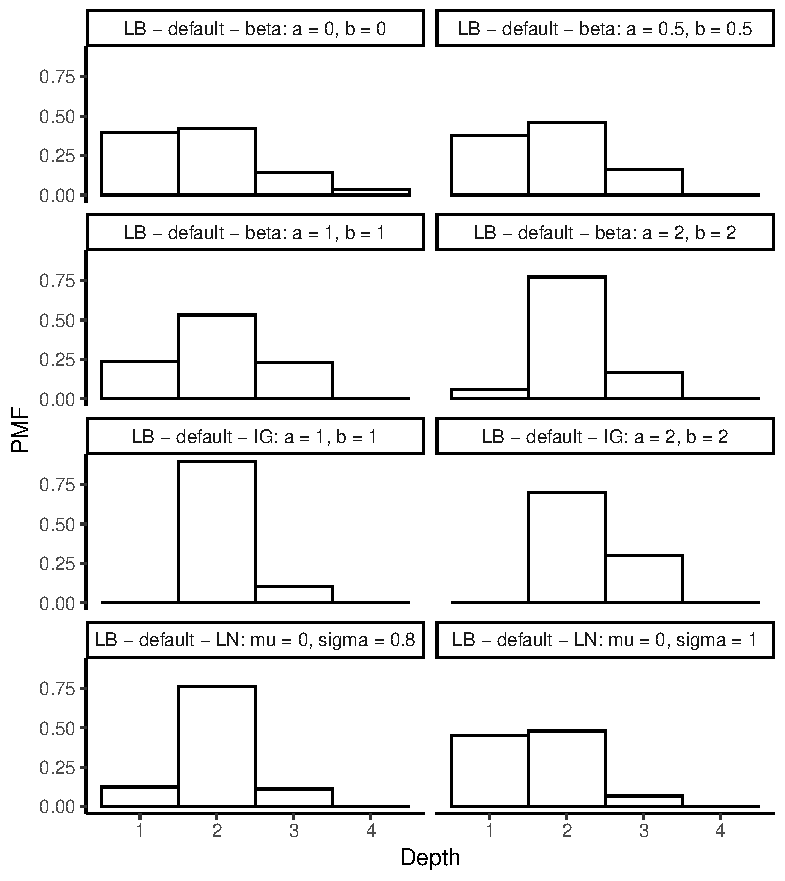
\includegraphics[width=0.95\linewidth]{hist_depth_4.pdf}
	\caption{Histogram of depth}
	\label{fig:hist:depth:4}
\end{figure}

\begin{figure}[ht]
	\centering
	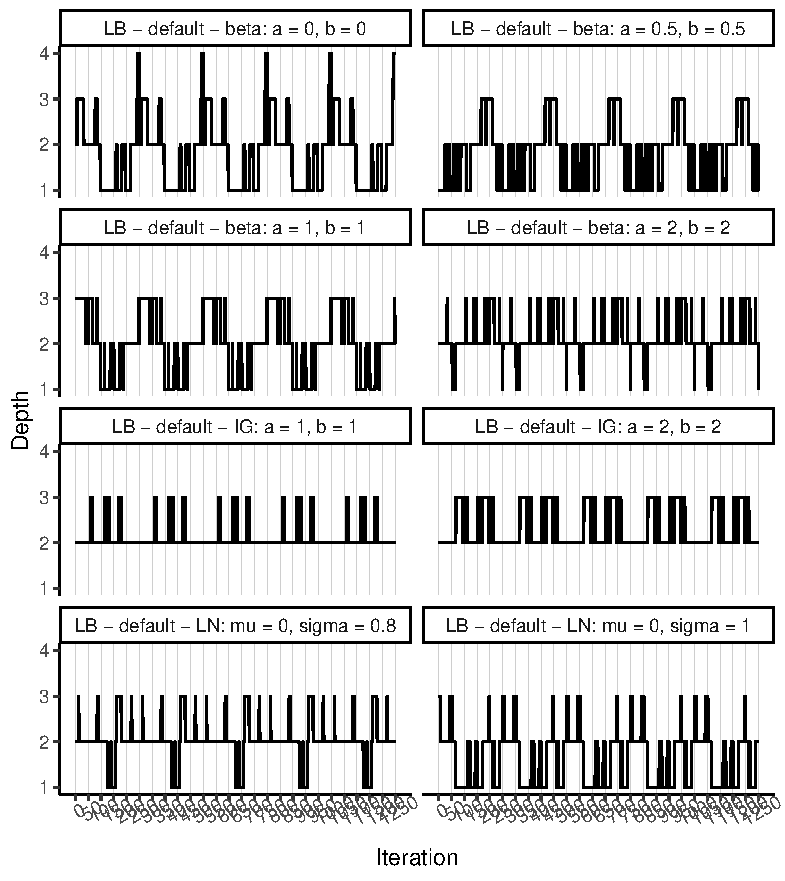
\includegraphics[width=0.95\linewidth]{trace_depth_4.pdf}
	\caption{Trace of depth}
	\label{fig:trace:depth:4}
\end{figure}

\begin{figure}[ht]
	\centering
	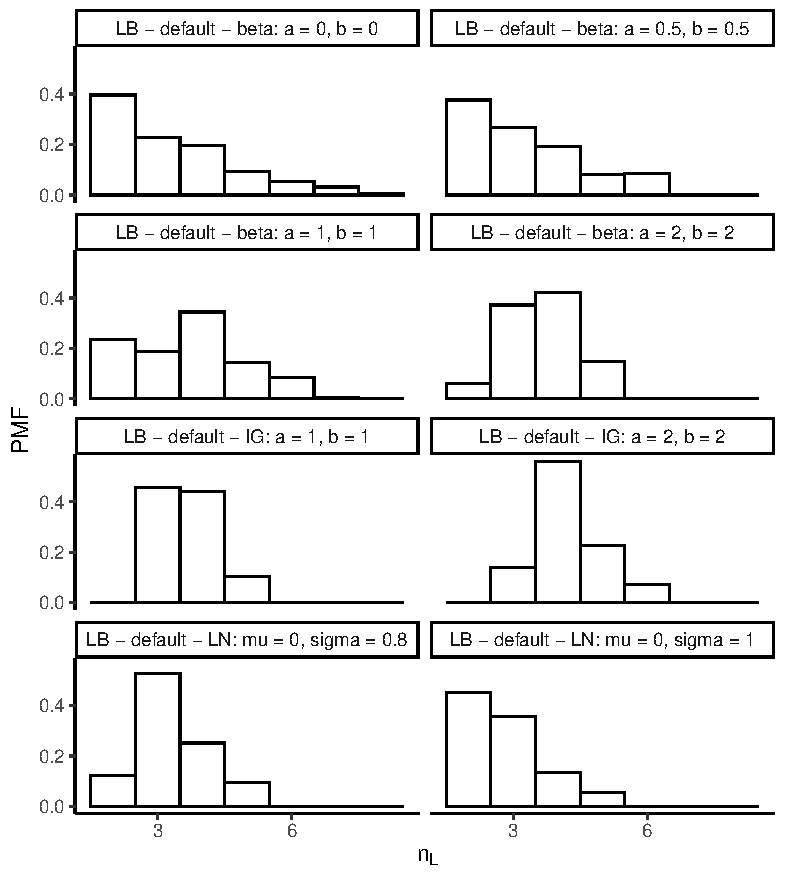
\includegraphics[width=0.95\linewidth]{hist_nl_4.pdf}
	\caption{Histogram of $n_L$}
	\label{fig:hist:nl:4}
\end{figure}

\begin{figure}[ht]
	\centering
	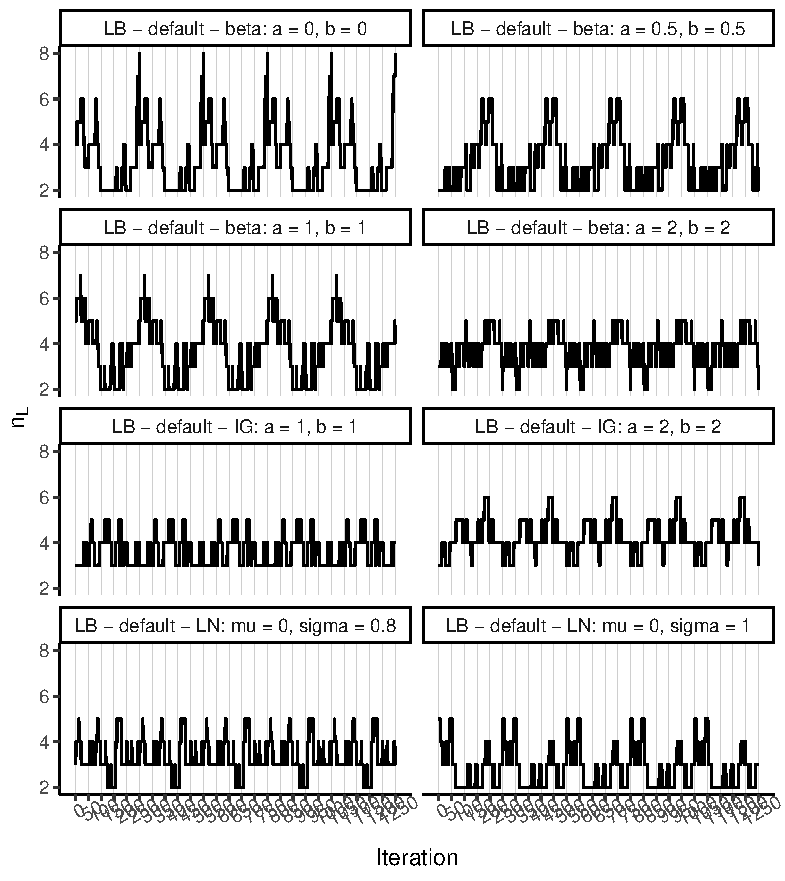
\includegraphics[width=0.95\linewidth]{trace_nl_4.pdf}
	\caption{Trace of $n_L$}
	\label{fig:trace:nl:4}
\end{figure}
\iffalse
\begin{figure}[ht]
	\centering
	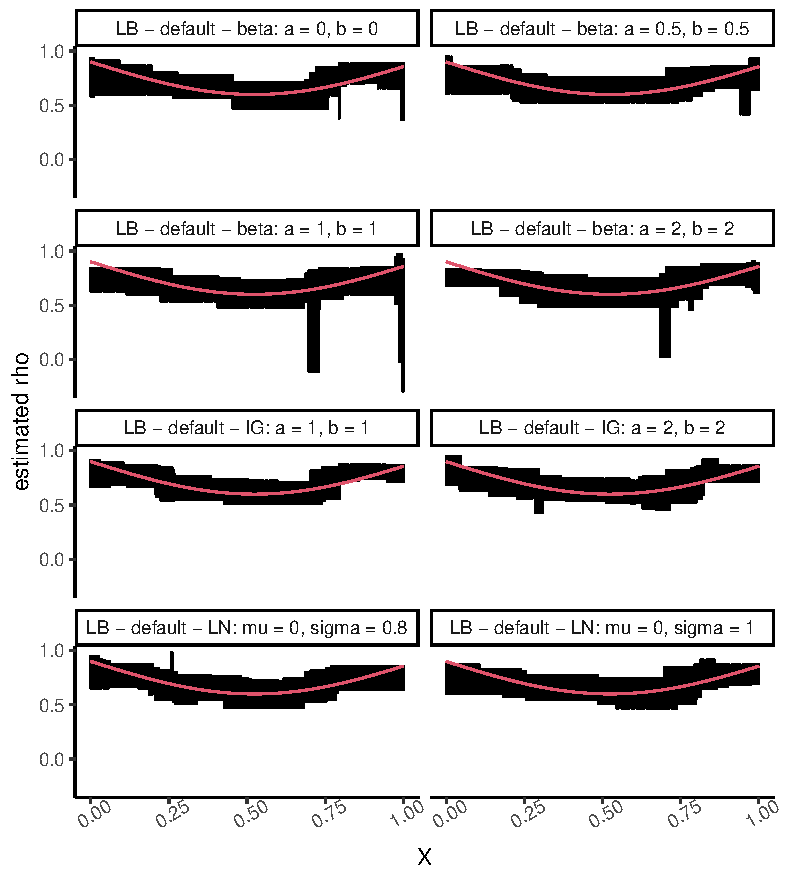
\includegraphics[width=0.95\linewidth]{mcmc_rho_4.pdf}
	\caption{MCMC of $\rho$}
	\label{fig:mcmc:rho:4}
\end{figure}
\fi
\begin{figure}[ht]
	\centering
	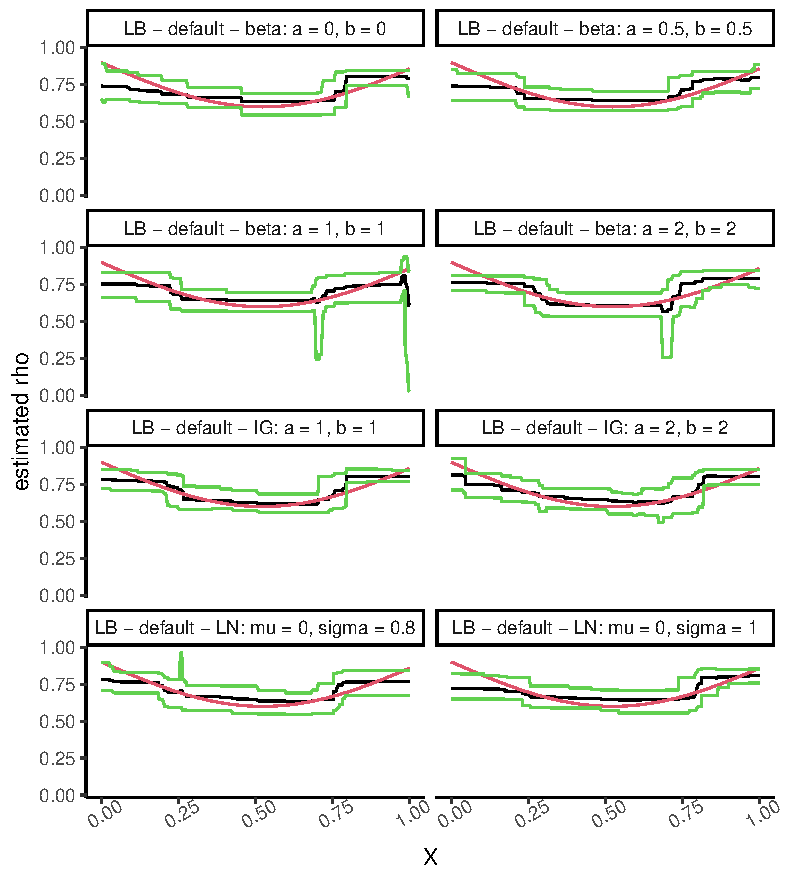
\includegraphics[width=0.95\linewidth]{predicted_rho_4.pdf}
	\caption{Estimated $\rho$ and credible intervals}
	\label{fig:pred:rho:4}
\end{figure}

\begin{figure}[ht]
	\centering
	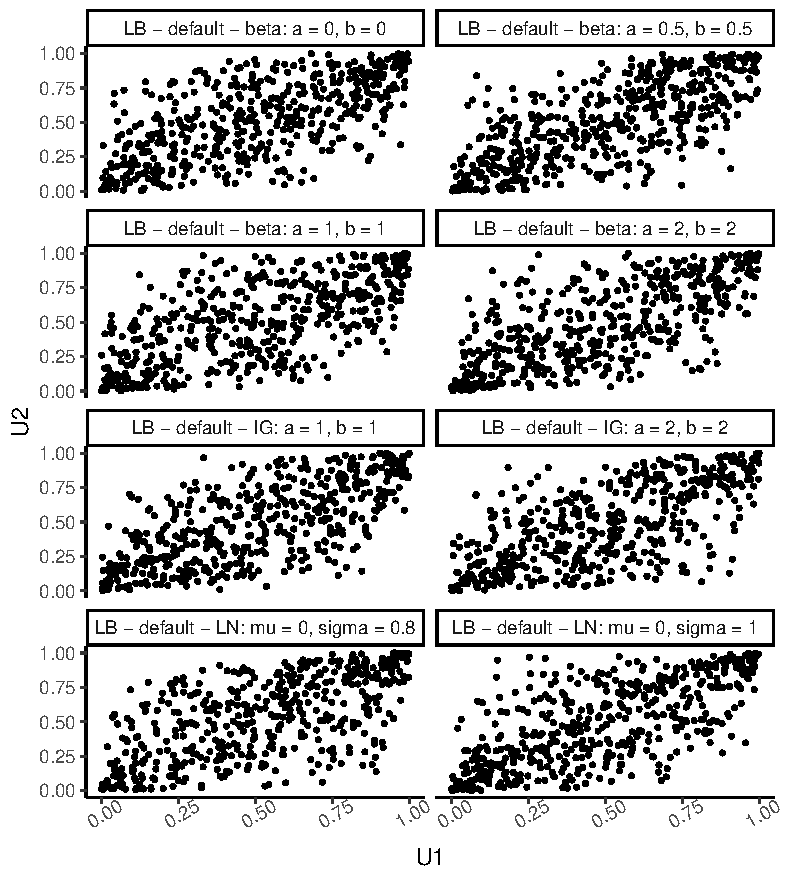
\includegraphics[width=0.95\linewidth]{simulated_copula_4.pdf}
	\caption{Predicted copula with estimated $\rho$}
	\label{fig:sim:copula:4}
\end{figure}

%
\begin{figure}[ht]
	\centering
	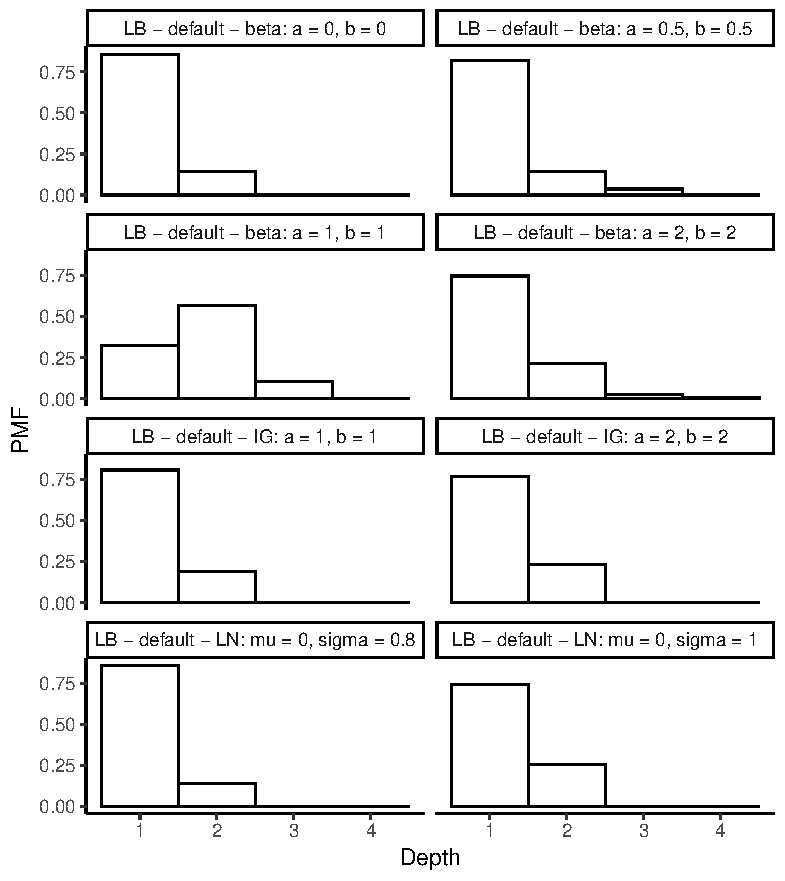
\includegraphics[width=0.95\linewidth]{hist_depth_5.pdf}
	\caption{Histogram of depth}
	\label{fig:hist:depth:5}
\end{figure}

\begin{figure}[ht]
	\centering
	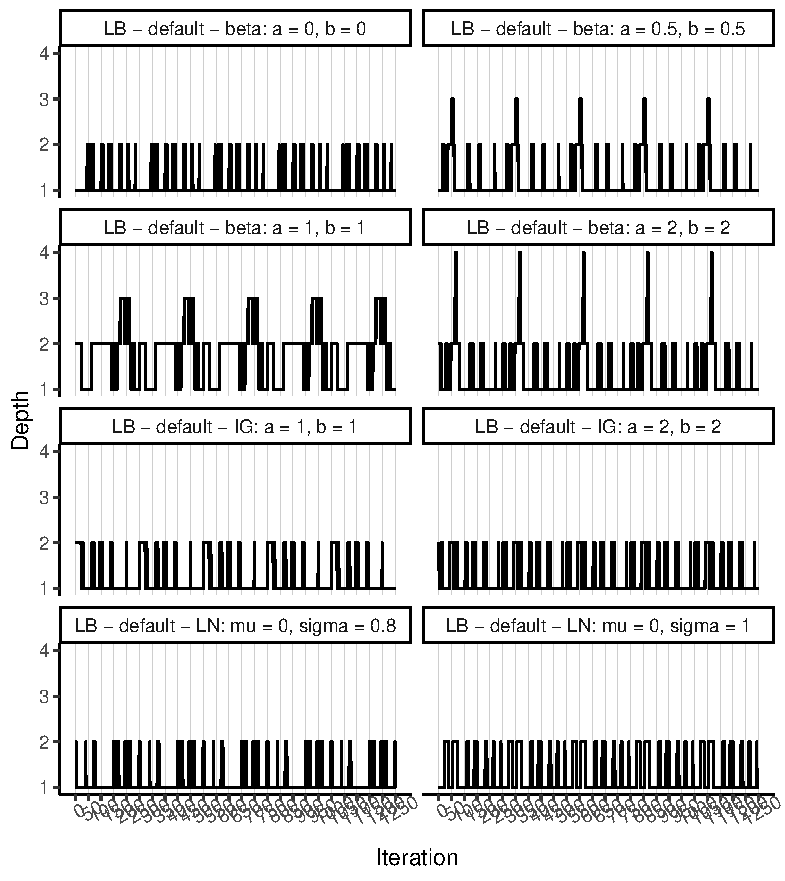
\includegraphics[width=0.95\linewidth]{trace_depth_5.pdf}
	\caption{Trace of depth}
	\label{fig:trace:depth:5}
\end{figure}

\begin{figure}[ht]
	\centering
	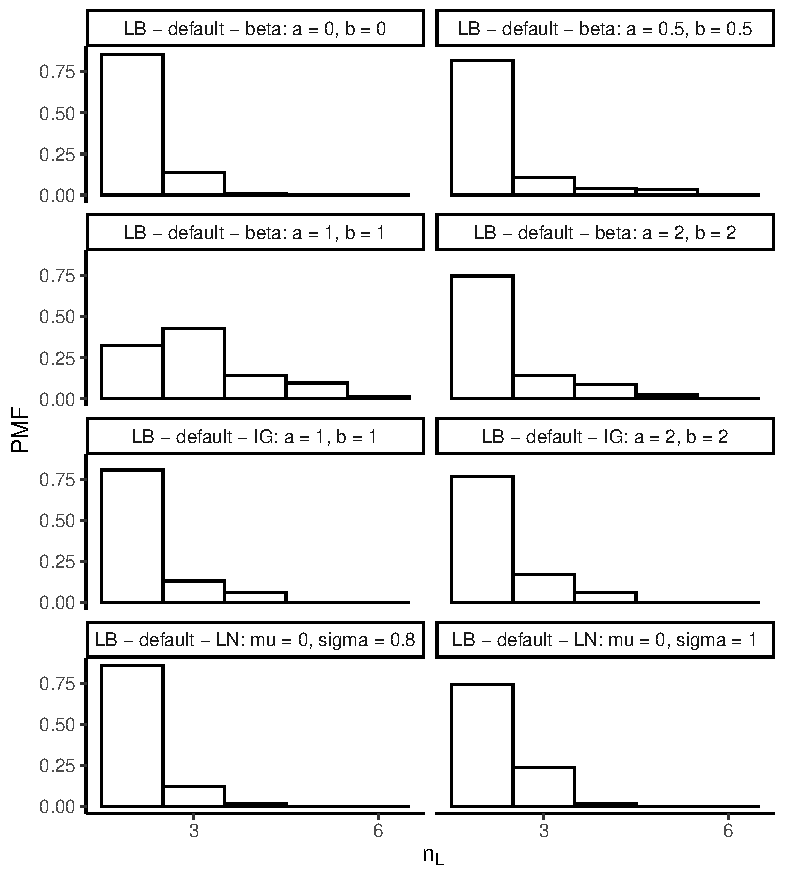
\includegraphics[width=0.95\linewidth]{hist_nl_5.pdf}
	\caption{Histogram of $n_L$}
	\label{fig:hist:nl:5}
\end{figure}

\begin{figure}[ht]
	\centering
	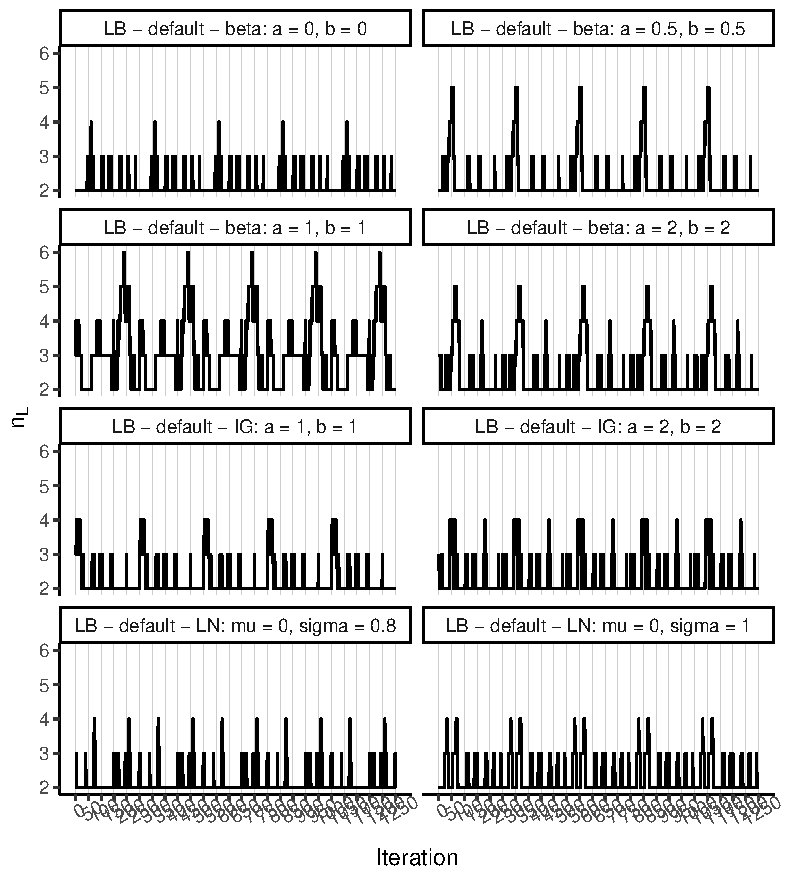
\includegraphics[width=0.95\linewidth]{trace_nl_5.pdf}
	\caption{Trace of $n_L$}
	\label{fig:trace:nl:5}
\end{figure}
\iffalse
\begin{figure}[ht]
	\centering
	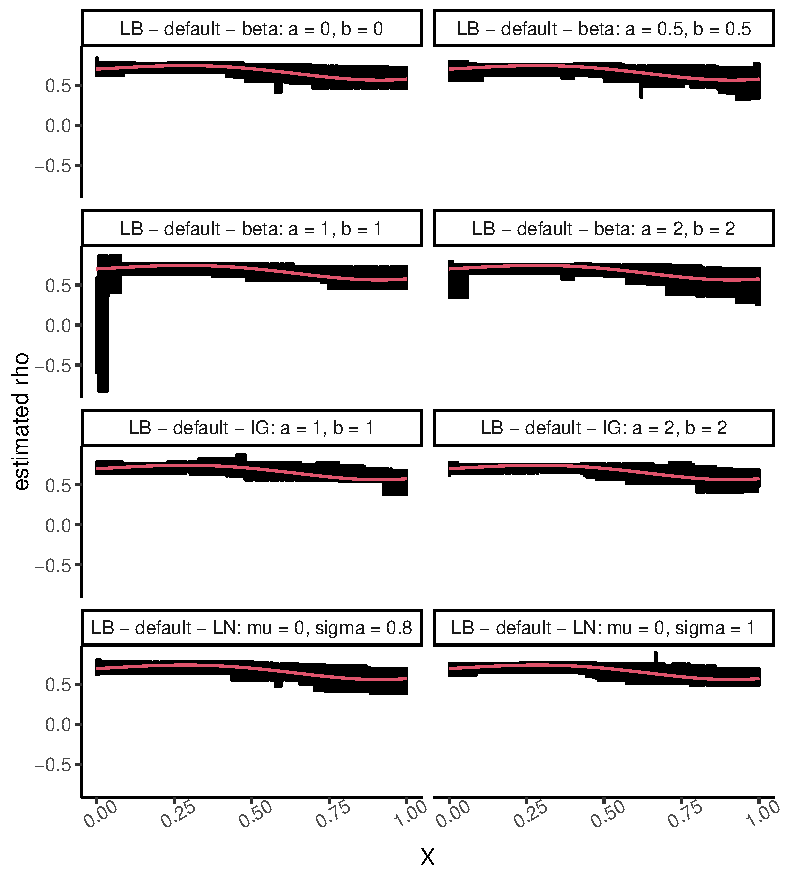
\includegraphics[width=0.95\linewidth]{mcmc_rho_5.pdf}
	\caption{MCMC of $\rho$}
	\label{fig:mcmc:rho:5}
\end{figure}
\fi
\begin{figure}[ht]
	\centering
	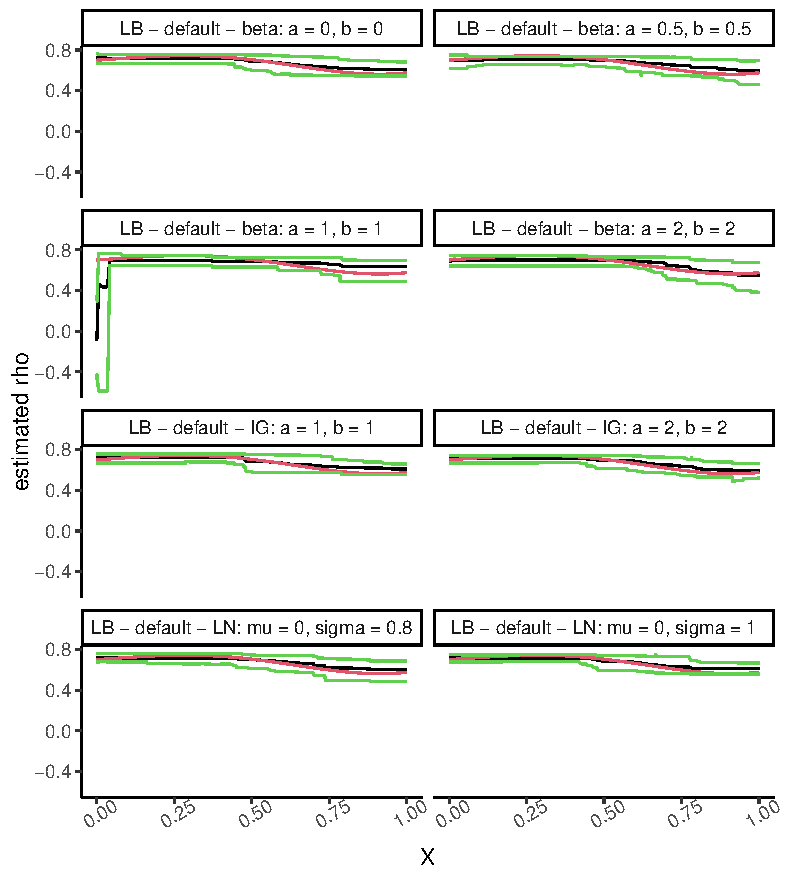
\includegraphics[width=0.95\linewidth]{predicted_rho_5.pdf}
	\caption{Estimated $\rho$ and credible intervals}
	\label{fig:pred:rho:5}
\end{figure}

\begin{figure}[ht]
	\centering
	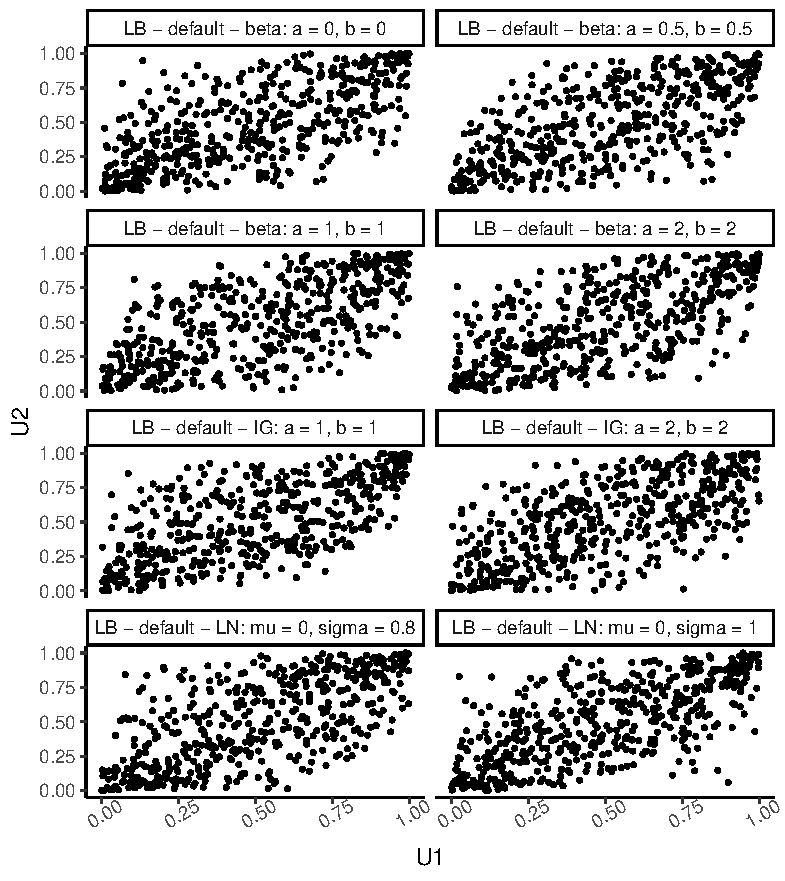
\includegraphics[width=0.95\linewidth]{simulated_copula_5.pdf}
	\caption{Predicted copula with estimated $\rho$}
	\label{fig:sim:copula:5}
\end{figure}


\end{document}
